%%    _____  _____
%%   |  __ \|  __ \    AUTHOR: Pedro Rivero
%%   | |__) | |__) |   ---------------------------------
%%   |  ___/|  _  /    DATE: April 27, 2020
%%   | |    | | \ \    ---------------------------------
%%   |_|    |_|  \_\   https://github.com/pedrorrivero
%%

% \documentclass[9pt, aspectratio=169]{beamer}
\documentclass[9pt, handout, aspectratio=169]{beamer}	% Skip \pause commands
\usetheme{PRRwide}
\usepackage{PRRmath}

% \setbeameroption{show notes}
% \setbeameroption{show only notes}

%% ----------------------------------------------------------------------------
%% FRONT-MATTER
%% ----------------------------------------------------------------------------

\title{Quantum Computation for the Understanding of Mass}
\subtitle{Simulating Quantum Field Theories}
\author{Pedro Rivero}
\institute{Illinois Institute of Technology \\ Argonne National Laboratory}
\newcommand{\mail}{priveroramirez@hawk.iit.edu}
\date{\today}
\newcommand{\website}{
	\href{https://www.iit.edu/physics}
	{www.iit.edu/physics}
}

\begin{document}
	\justify
	\setlength{\abovedisplayskip}{0pt}
	\setlength{\belowdisplayskip}{12pt}
	\setlength{\abovedisplayshortskip}{0pt}
	\setlength{\belowdisplayshortskip}{12pt}

\begin{frame}[plain,t]
	\titlepage
\end{frame}

% \begin{frame}[c]{Contents}
% %		\begin{multicols}{2}
% %  			\tableofcontents
% %		\end{multicols}
% 	\tableofcontents
% \end{frame}


%% ----------------------------------------------------------------------------
%% MAIN-MATTER
%% ----------------------------------------------------------------------------

\section{Introduction}

\begin{frame}{Introduction}

	Nature is described through the mathematical framework provided by \textbf{Quantum Field Theory}.

	\begin{multicols}{2}

		\begin{itemize}
			\item<2-> The different implementations of Quantum Field Theory are referred to as quantum field theories themselves.
			\item<3-> Quantum Chromodynamics (QCD) is the theory of the strong nuclear force.
			\item<3-> QCD holds many mysteries (e.g. \textbf{mass generation} phenomena).
			\item<4-> QCD is currently studied using brute-force numerics on the world’s largest supercomputers.
			\item<4-> Many aspects of quantum field theories cannot be studied using classical computers.
		\end{itemize}

		\begin{center}
			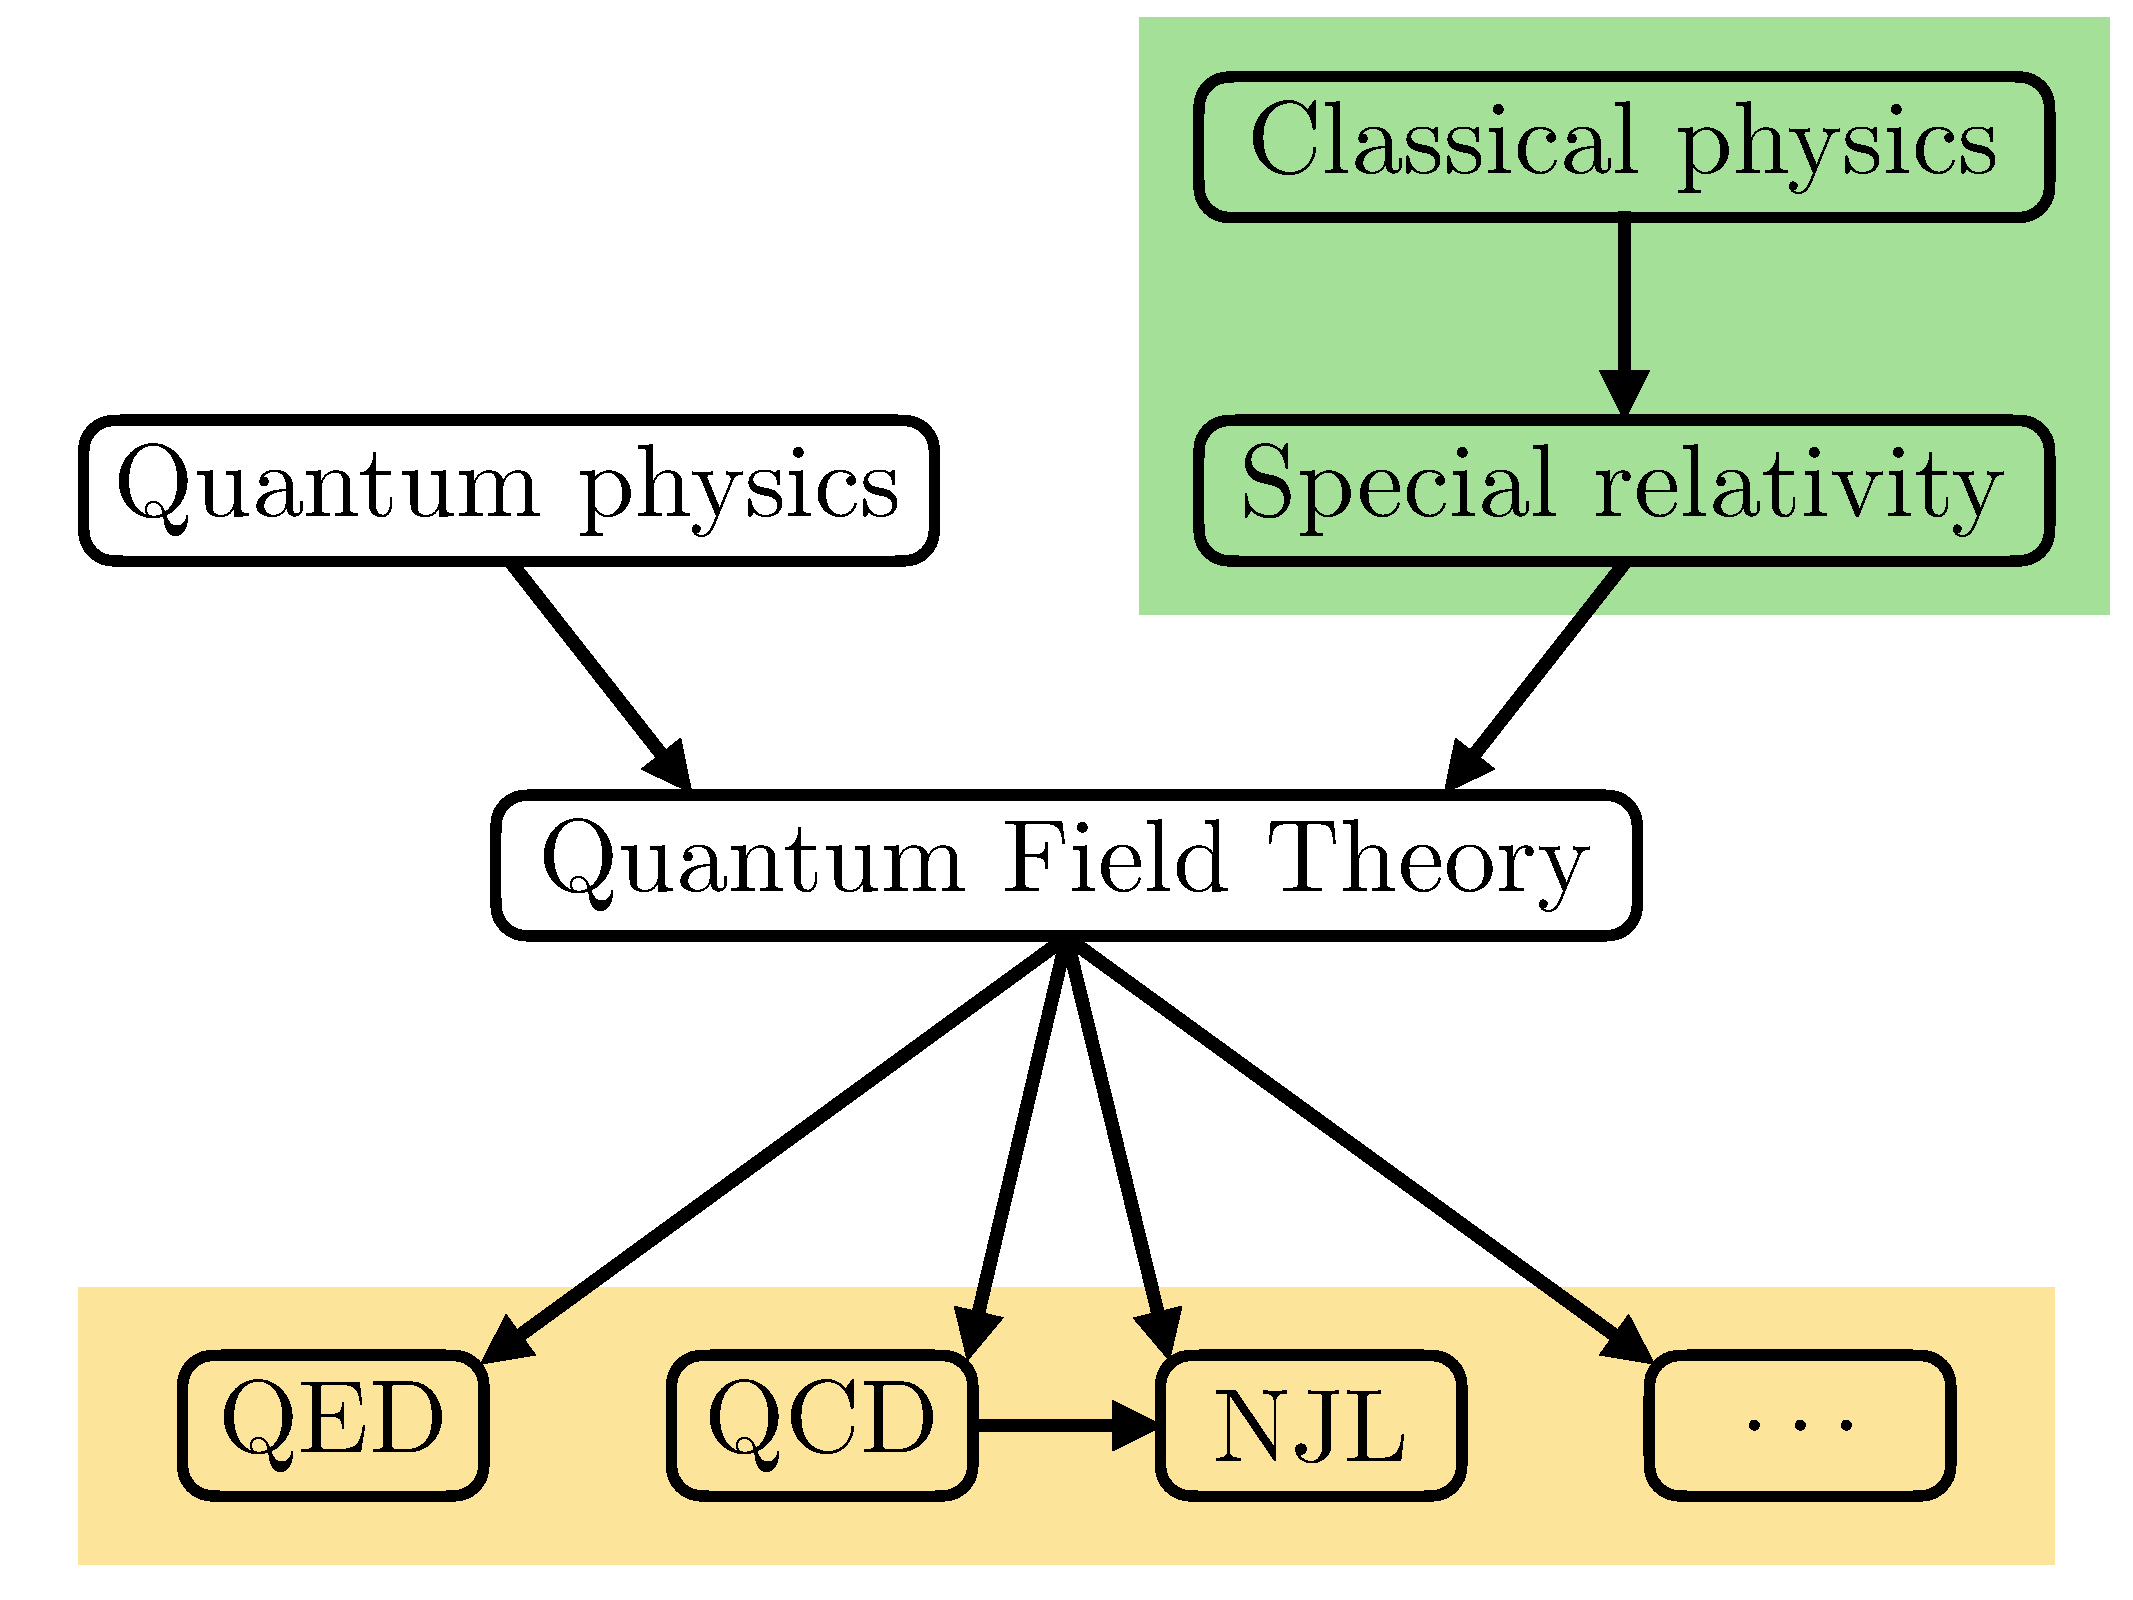
\includegraphics[width=.40\paperwidth]{Figures/quantum-field-theory}
		\end{center}

	\end{multicols}

\end{frame}

%% ----------------------------------------------------------------------------

\begin{frame}{Objectives}

	An important path forward is to develop methods to simulate these models on quantum computers. This effort is only just beginning, however, performing calculations on a quantum computer is far from being a straightforward task; and it has only been achieved for relatively simple problems. My goal will be to develop some of the techniques necessary to use quantum computers for this endeavor. We will do so by analyzing the following:

	\medskip

	\begin{itemize}
		\item<2-> \textbf{Nambu--Jona-Lasino model} (NJL) in $1+1$ dimensions: an effective field theory, regarded as a low-energy approximation to QCD.
		\item<3-> It retains certain key features of QCD, such as the so called Goldstone modes and \textbf{dynamical chiral symmetry breaking}; which in turn is responsible for the creation of dressed mass.
		\item<4-> This model can be solved nonperturbatively through the standard leading order truncation; an important characteristic since verifying the solutions returned by any quantum computation is currently a major challenge.
	\end{itemize}

\end{frame}

%% ----------------------------------------------------------------------------

\begin{frame}[c]{Contents}
%		\begin{multicols}{2}
%  			\tableofcontents
%		\end{multicols}
	\tableofcontents
\end{frame}

%% ----------------------------------------------------------------------------
%% ----------------------------------------------------------------------------

\section{Background in Quantum Computation}

\begin{frame}{Background in Quantum Computation}

	Before the abacus was invented, the only way of counting was through a "thermometer-like" scale. This device introduced the concept of \textbf{digits}, which was later adopted into our own language in the form of \textbf{numerals}. This meant that, instead of counting up to $N$ using $N$ elements, we could count using only $\text{log}_b (N)$ abacus elements ---where $b$ is the base of our number system (i.e. the amount of beads per row in the abacus).

		\begin{multicols}{2}

		 	Therefore, for $b\geq2$, the abacus introduced an \textbf{exponential decrease in resource requirements}.

			\medskip

			Quantum computers do something analogous. To represent the quantum state of a system made out of $N$ subsystems ---with $b$ degrees of freedom each--- we would usually need $b^N$ classical elements (i.e. numbers). By using quantum systems for this representation, we would only need $N$ quantum elements (i.e. each subsystem).

			\columnbreak

			\begin{center}
				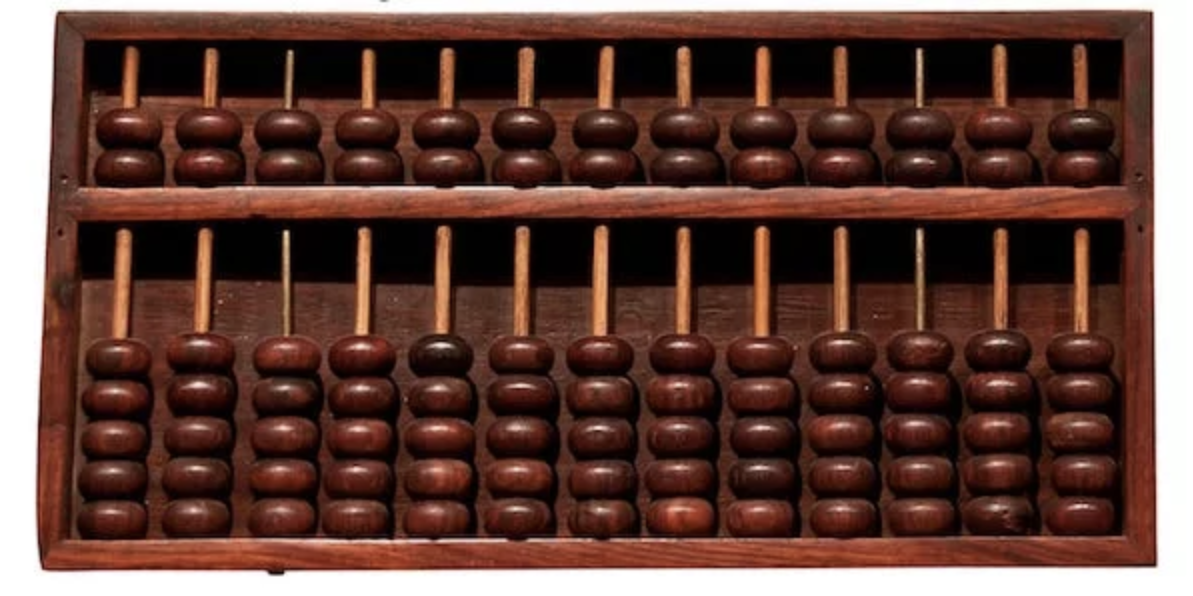
\includegraphics[width=.30\paperwidth]{Figures/abacus} \\
				\vspace{10pt}
				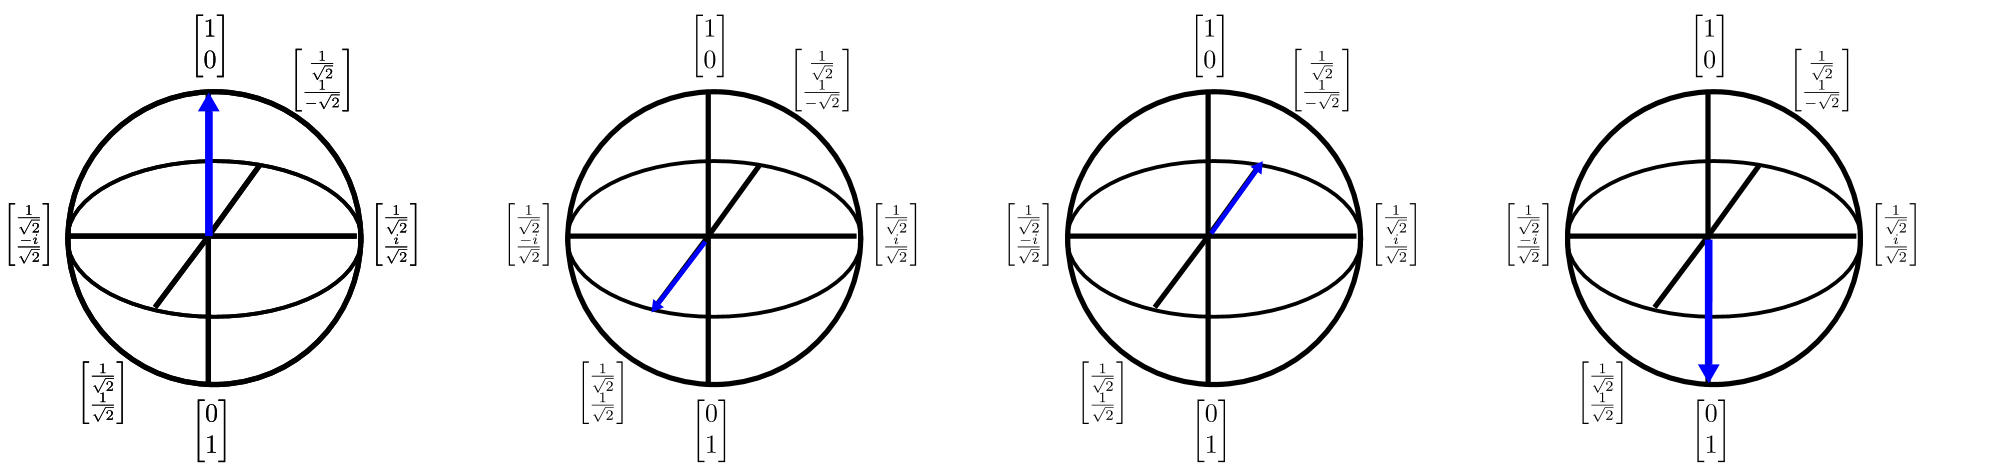
\includegraphics[width=.34\paperwidth]{Figures/qubits}
			\end{center}

		\end{multicols}

\end{frame}

%% ----------------------------------------------------------------------------

\subsection{Quantum logic}

\begin{frame}{Quantum logic}

	Formally speaking, the states of a quantum system will be represented as a vector in a Hilbert space; whereas the state of a classical system is simply an element of a set. This distinction, along with the probabilistic nature of quantum mechanics, makes the entire logical system describing quantum computers fundamentally different than \textbf{classical propositional logic} (i.e. Boolean algebra).

	% Because these logical systems are so different from each other, if we are to take advantage of the power of quantum mechanics for performing computations, it is essential to “think” in quantum terms; and formulate the problems that we want to solve according to this new logic.

	\begin{multicols}{2}

		\action<2->{
			\underline{\textbf{CLASSICAL LOGIC}}\\
			\small{\emph{Set Theory (Boolean algebra)}}

			\medskip

			\begin{itemize}
				\item \textbf{AND} $\quad \Rightarrow \quad A \cup B$
				\item \textbf{OR} $\quad \Rightarrow \quad A \cap B$
				\item \textbf{NOT} $\quad \Rightarrow \quad \overline{A}$
				\item \textbf{XOR} $ \quad \Rightarrow \quad A \cap B - A \cup B$
			\end{itemize}
		}

		\columnbreak

		\action<3->{
			\underline{\textbf{QUANTUM LOGIC}}\\
			\small{\emph{Quantum Theory (Non-abelian)}}

			\medskip

			\begin{itemize}
				\item \textbf{Probabilistic measurement}
				\item \textbf{Measurement causes disturbance}
				\item \textbf{Superposition}
				\item \textbf{Entanglement}
				\item \textbf{Uncertainty principle}
			\end{itemize}
		}

	\end{multicols}

\end{frame}

%% ----------------------------------------------------------------------------

\begin{frame}{Bloch sphere representation of a qubit}

	\begin{multicols}{2}

		The basic unit of information in quantum mechanics is the \textbf{qubit}; a quantum system with only two distinguishable states: $\ket{0}$ and $\ket{1}$.

		\medskip

		The main difference between bit and qubit lays in the fact that, when they are not being measured, quantum systems do not need to be in one of their so called, mutually incompatible, basis states; instead, they can be in any (normalized) \textbf{linear superposition} of them.

		\medskip

		A simple example of a qubit is a spin-$\frac{1}{2}$ particle; whose space of states is spanned by the spin up and spin down quantum basis. Inspired by this particular system, the qubit can be pictorially represented through the \textbf{Bloch sphere}.

		% This allows us to visualize non-commutative quantum logic.

		\columnbreak

		\begin{center}
			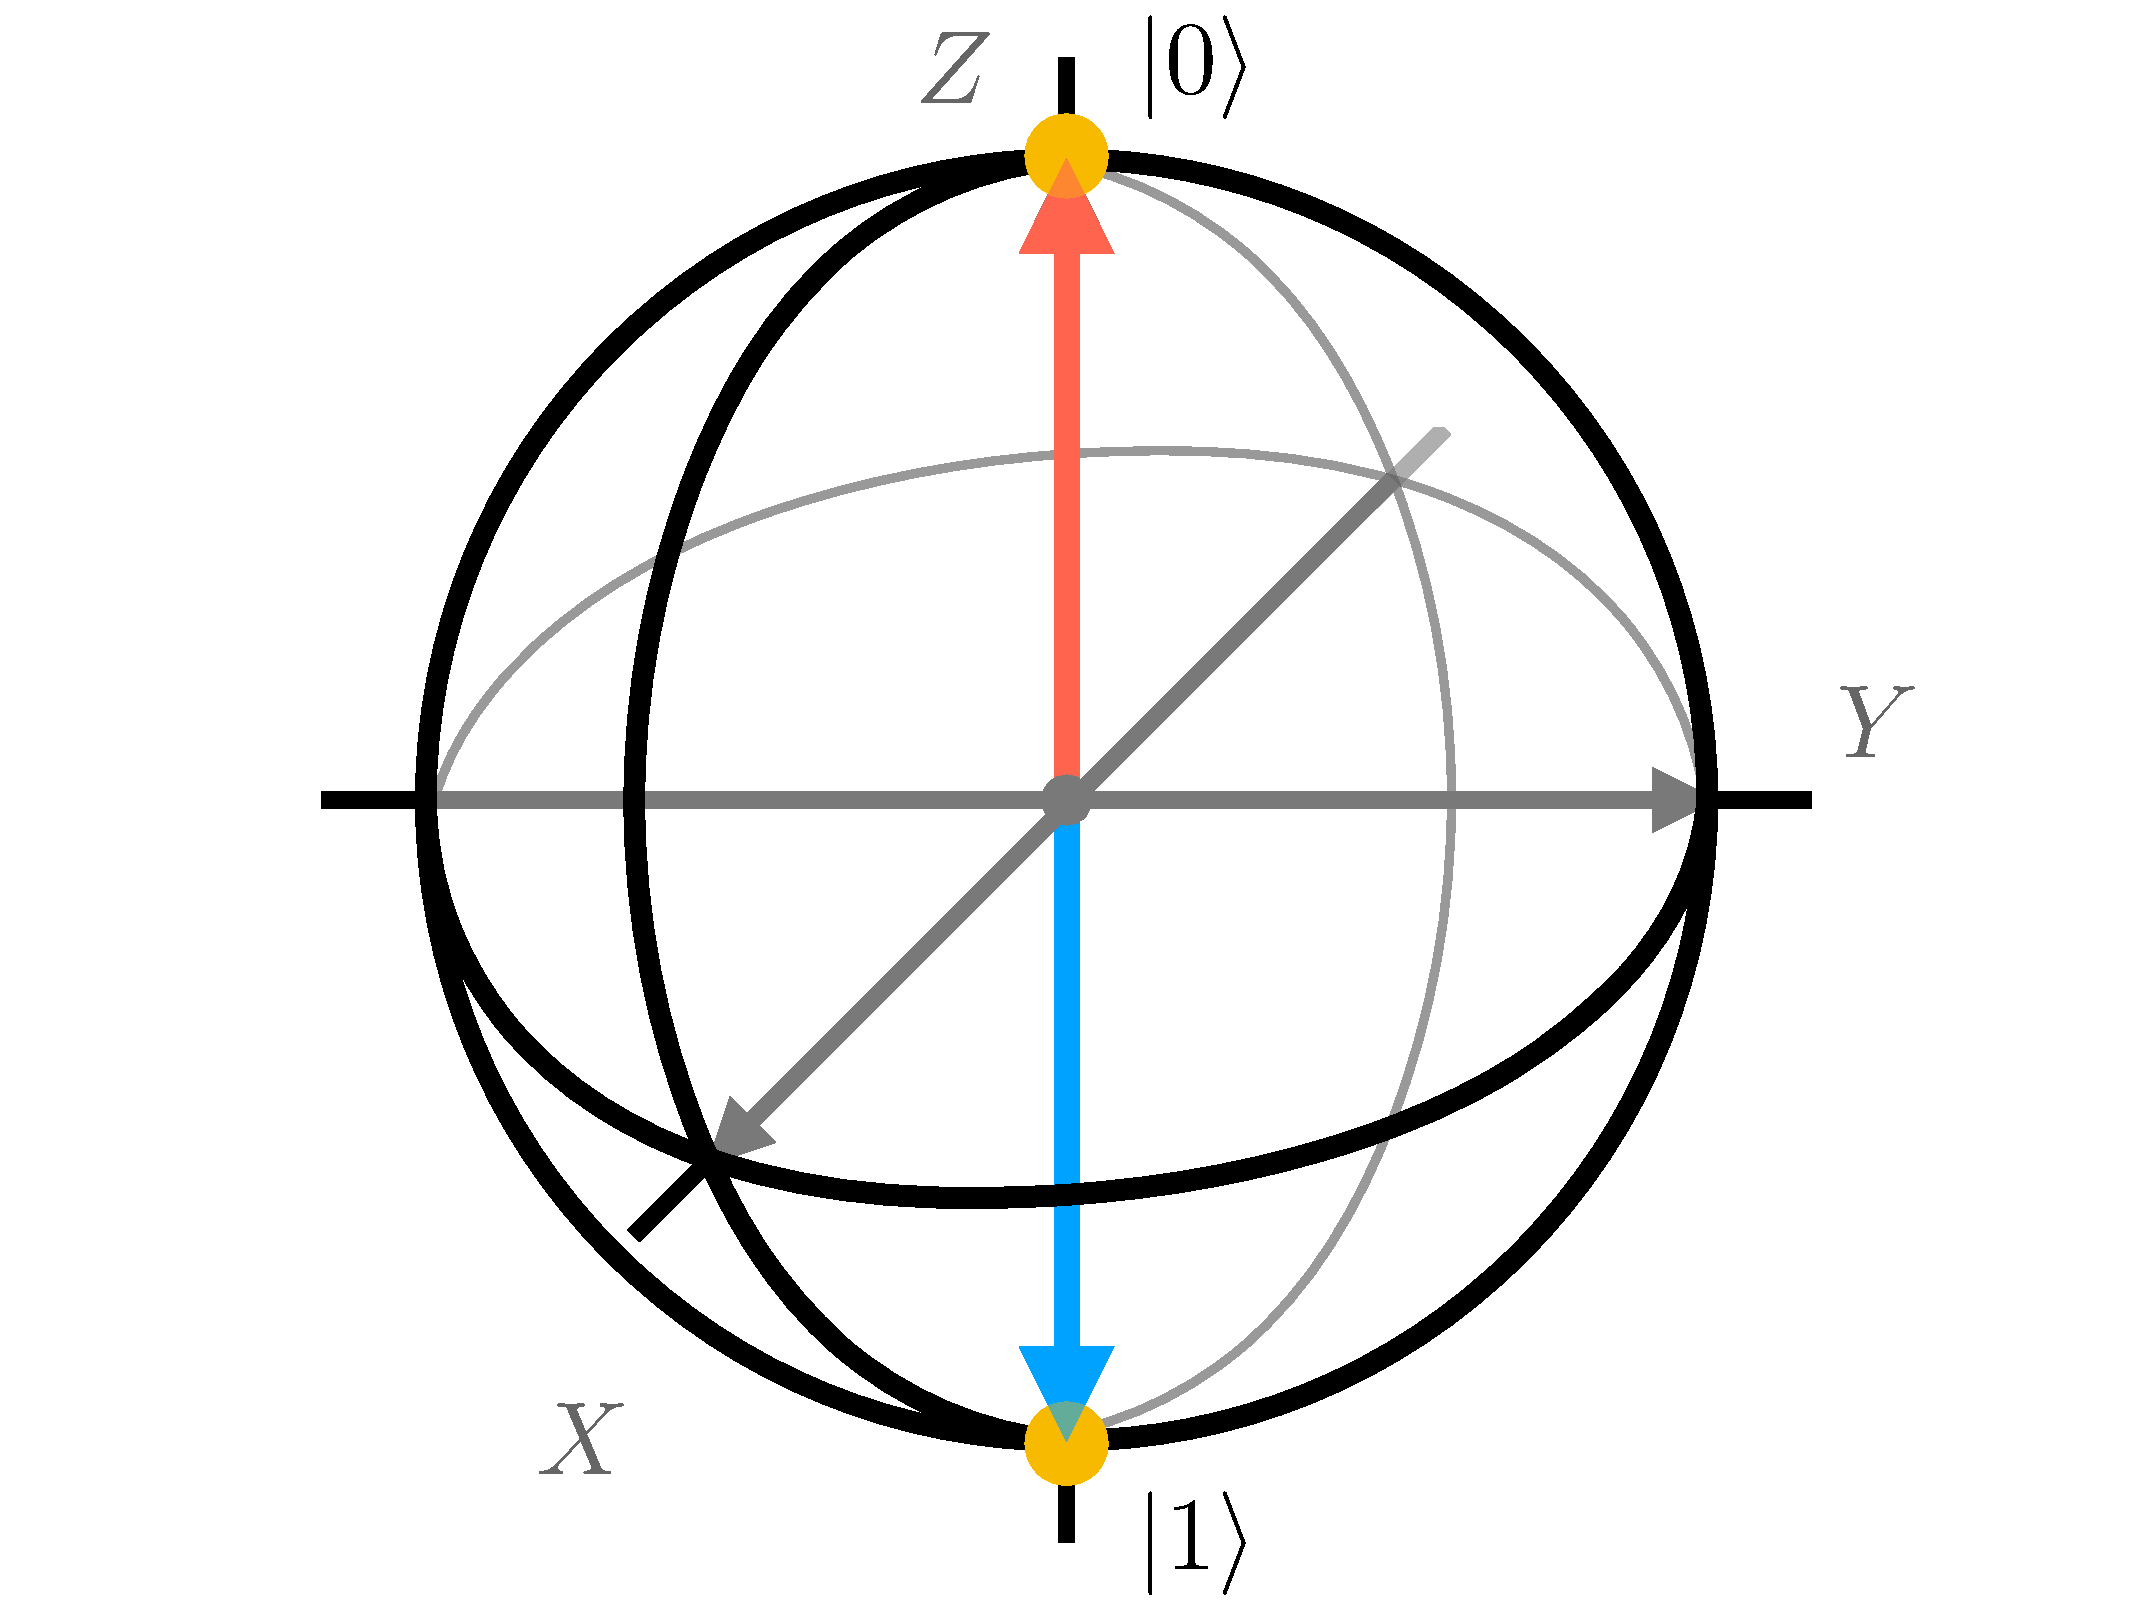
\includegraphics[width=.40\paperwidth]{Figures/quantum-background/bloch-sphere}
		\end{center}

	\end{multicols}

\end{frame}

%% ----------------------------------------------------------------------------

\subsection{Quantum information}

\begin{frame}{Quantum information}

	In the same way that the device known as an abacus had its theoretical counterpart in positional number systems, quantum computers have Quantum Information Science (QIS); which help us understand the full capabilities of these new machines. Two very important insights extracted from QIS, and with direct applicability to quantum apparatuses are:

	\medskip

	\begin{itemize}
		\item<2-> \textbf{Unitary quantum state transformations} (i.e. reversible):\\
			\begin{gather*}
			  \braket{\psi_0}{\phi_0} \equiv \braket{\psi(t)}{\phi(t)} =
					\mel{\psi_0}{U^\dagger U}{\phi_0} \qRa U^\dagger U \equiv \mathds{1}
			\end{gather*}
		\item<3-> \textbf{No-cloning theorem}:\\
			\begin{gather*}
			  U_\text{cloning} \qty(\ket{\psi}_A \otimes \ket{e}_B) =
			    \ket{\psi}_A \otimes \ket{\psi}_B \qc
				U_\text{cloning} \qty(\ket{\phi}_A \otimes \ket{e}_B) =
			    \ket{\phi}_A \otimes \ket{\phi}_B \\
			\end{gather*}
			\vspace{-3em}
			\begin{align*}
				\braket{\psi}{\phi} &=
					\qty(\braket{\psi}{\phi})_A \qty(\braket{e}{e})_B =
					\qty(\bra{\psi}_A\otimes\bra{e}_B) \qty(\ket{\phi}_A\otimes\ket{e}_B) \\
				&\equiv \qty(\bra{\psi}_A\otimes\bra{e}_B)
						U_\text{cloning}^\dagger U_\text{cloning}
						\qty(\ket{\phi}_A\otimes\ket{e}_B) =
					\qty(\bra{\psi}_A\otimes\bra{\psi}_B)
						\qty(\ket{\phi}_A\otimes\ket{\phi}_B) \\
				&= \qty(\braket{\psi}{\phi})_A \qty(\braket{\psi}{\phi})_B =
					\qty(\braket{\psi}{\phi})^2
			\end{align*}
	\end{itemize}

\end{frame}

%% ----------------------------------------------------------------------------

\begin{frame}{Implications for quantum information technologies}

	The fact that all transformations have to preserve information (i.e. entropy), imply that they are unitary. This is the only kind of transformations that a quantum computer will be able to reproduce ideally. On the other hand, the no-cloning theorem can be used to construct inherently secure communication and data storage systems. Furthermore, it means that \textbf{superluminal communication} is impossible:

	\vspace{-2em}

	\begin{multicols}{2}

		\pause
		\begin{center}
			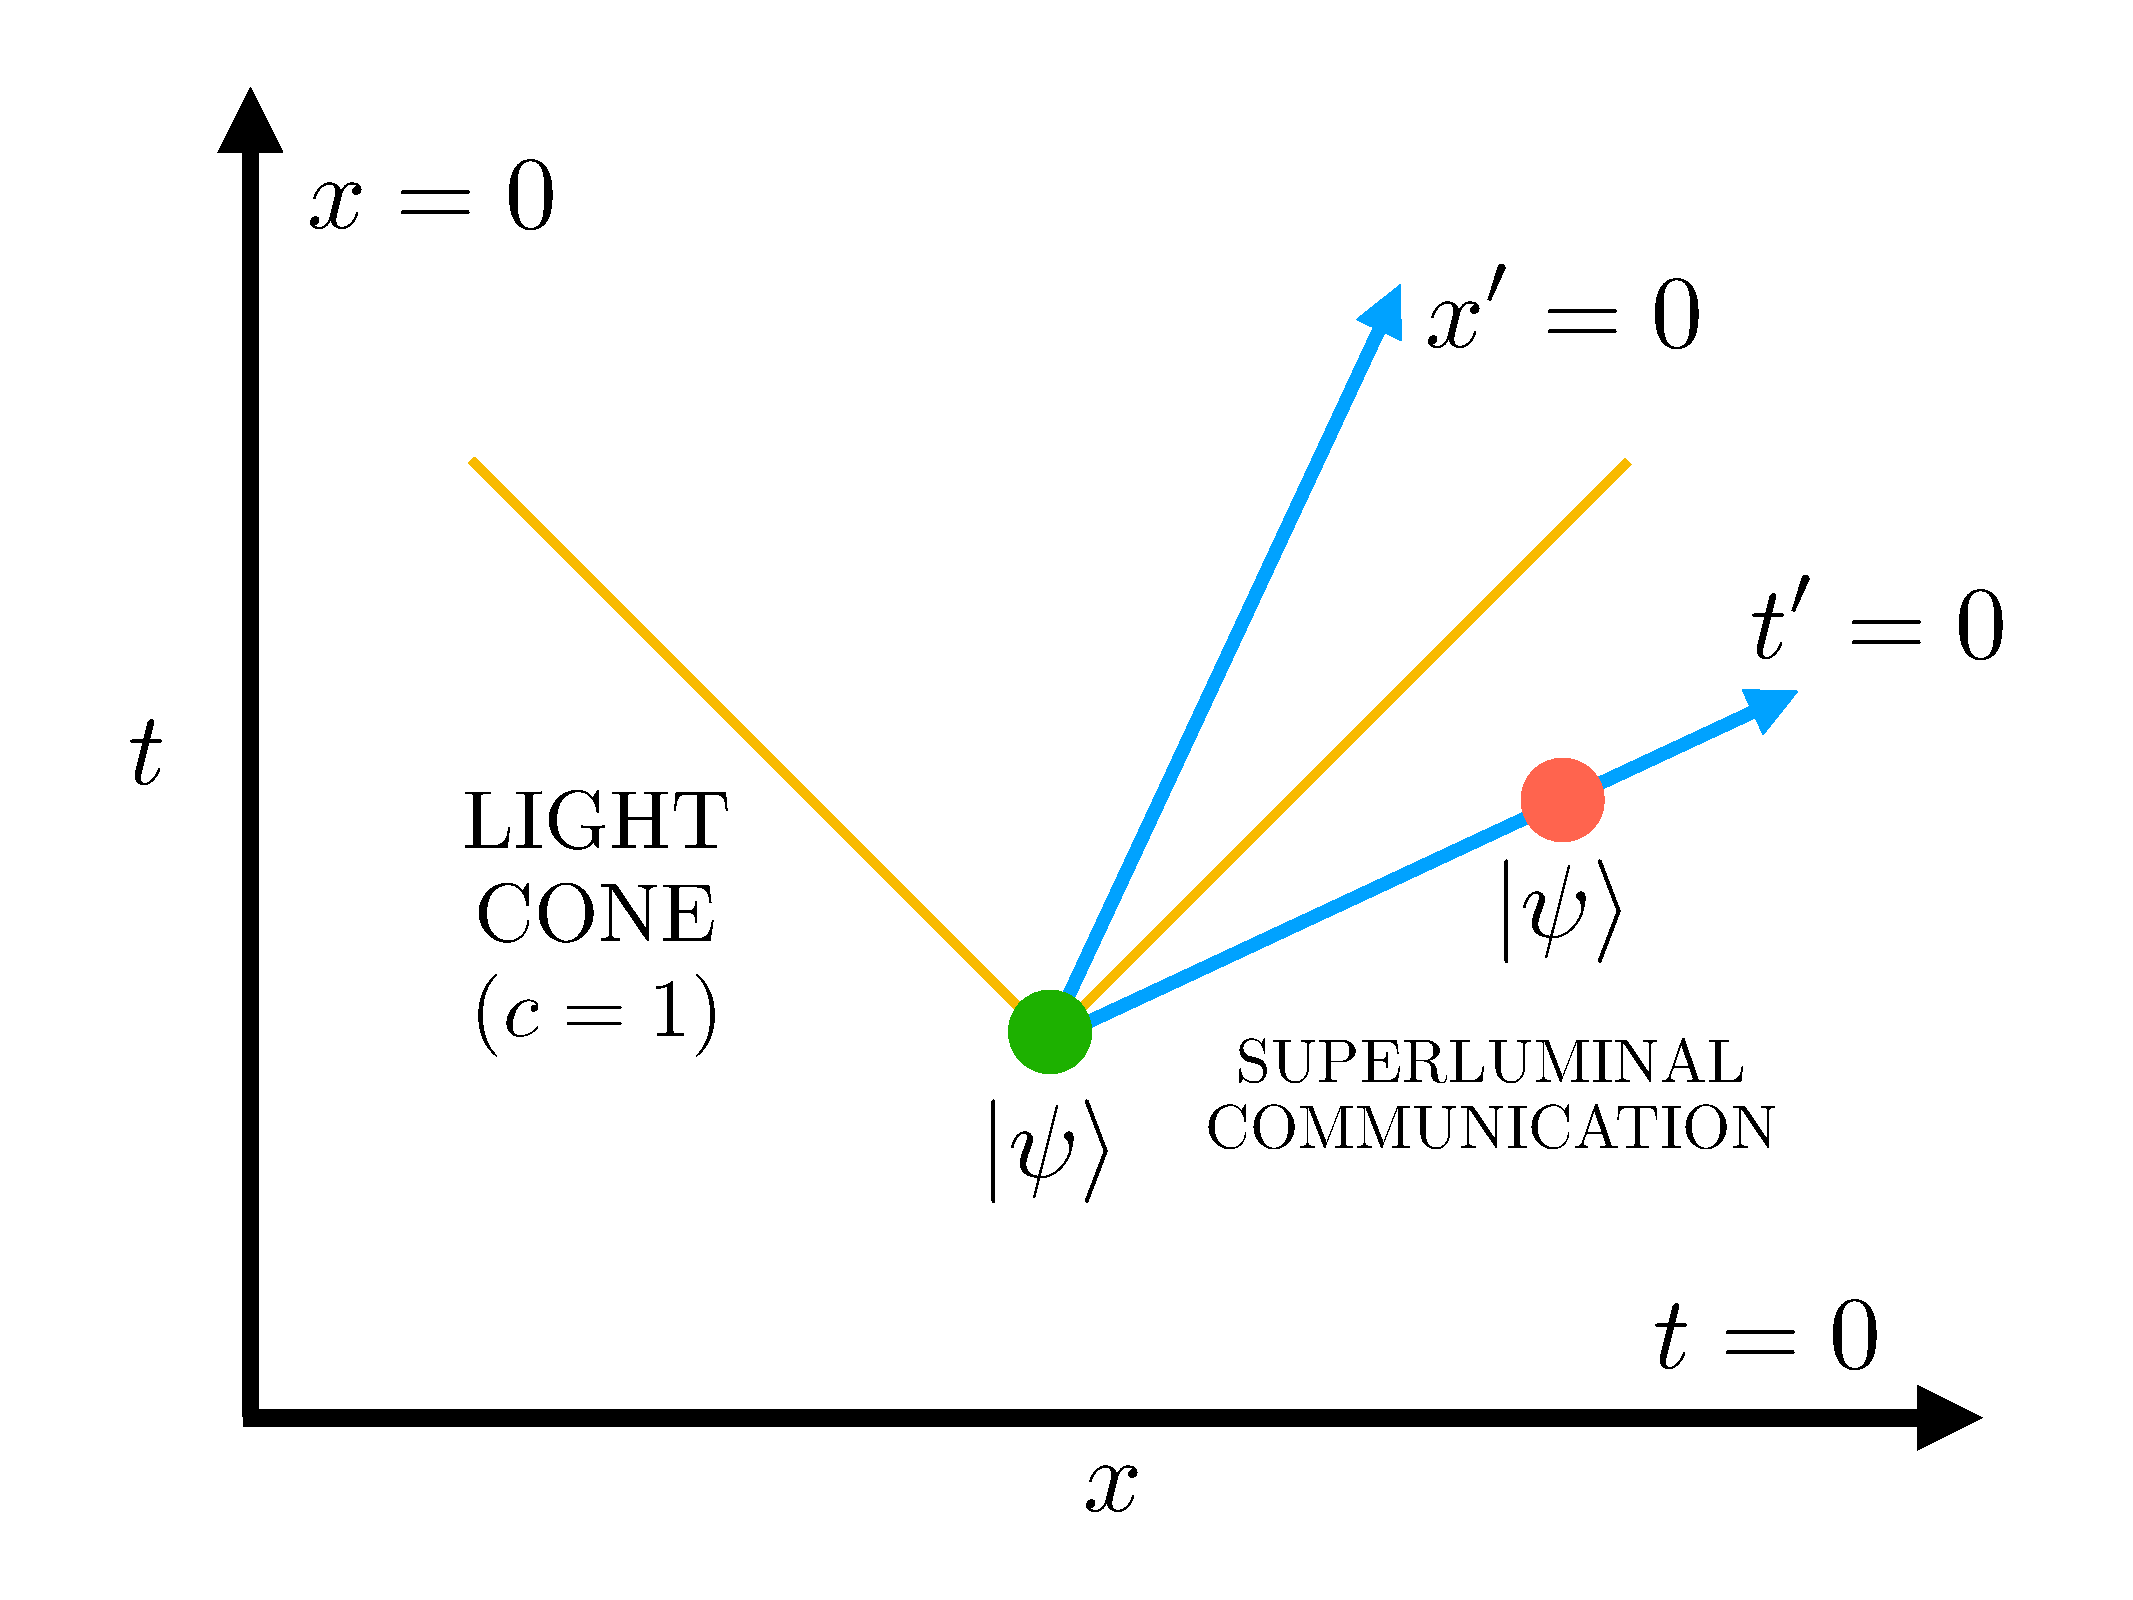
\includegraphics[width=.40\paperwidth]{Figures/quantum-background/superluminal-cloning-boost}
		\end{center}

		\columnbreak

		\pause
		\begin{center}
			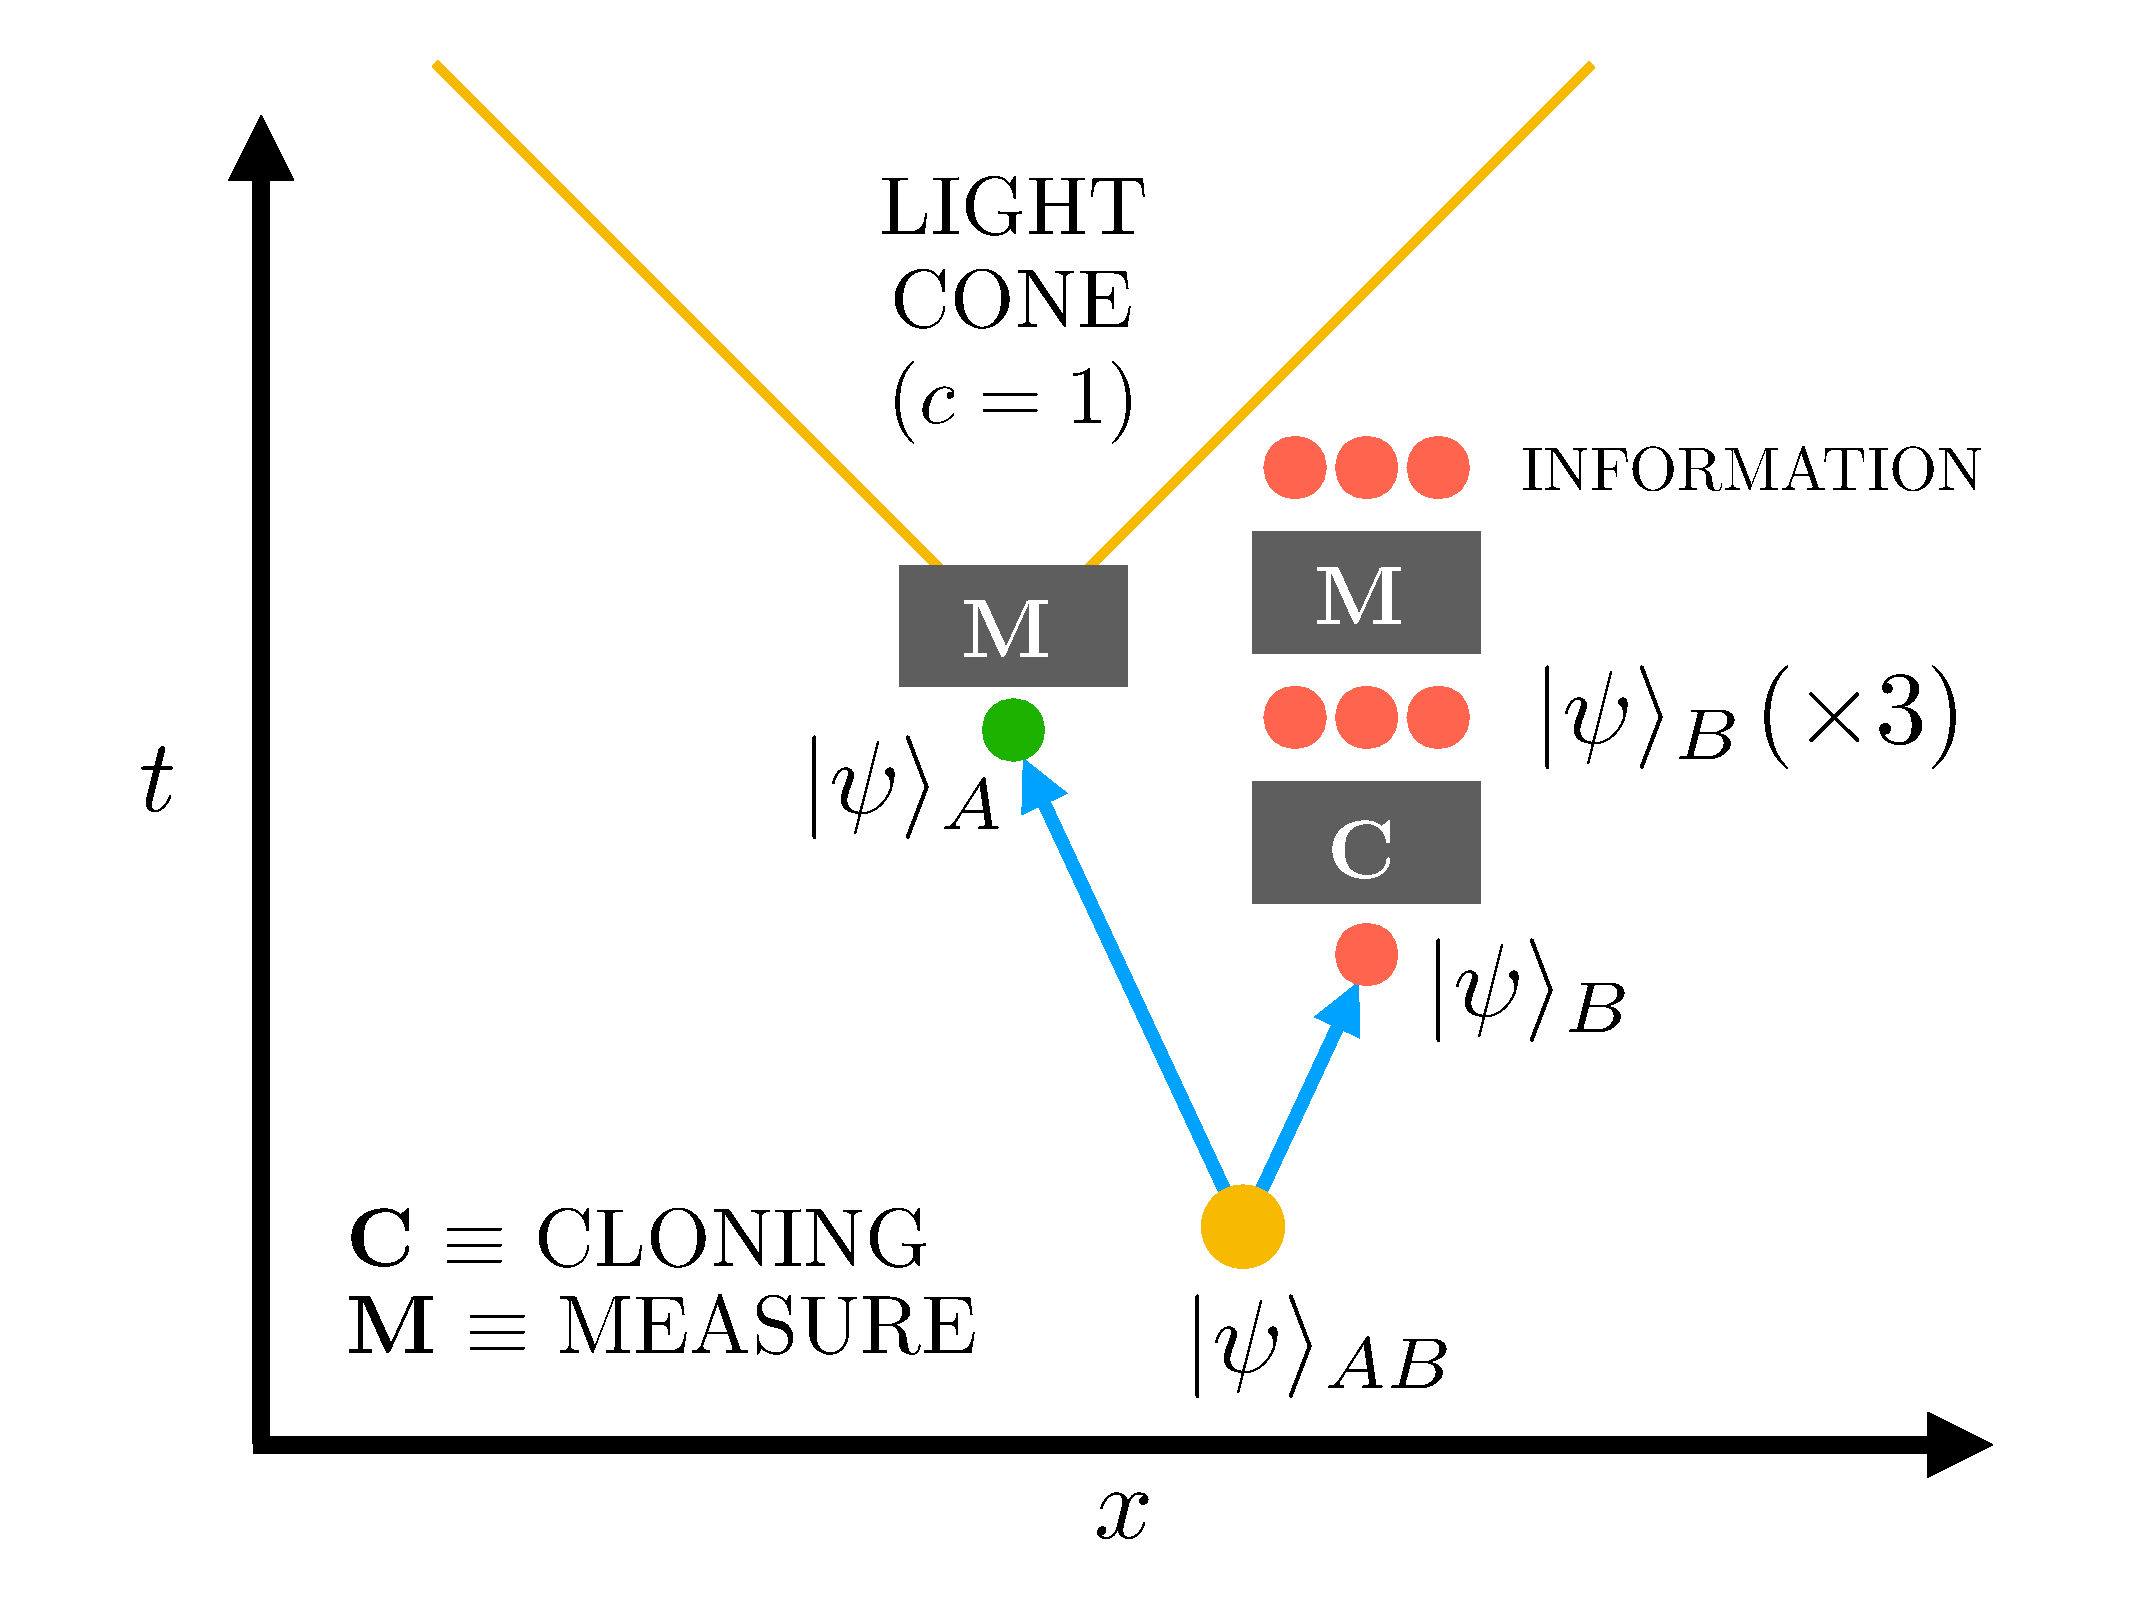
\includegraphics[width=.40\paperwidth]{Figures/quantum-background/superluminal-cloning-communication}
		\end{center}

	\end{multicols}

\end{frame}

%% ----------------------------------------------------------------------------

\subsection{Quantum circuits and quantum algorithms}

\begin{frame}{Quantum circuits and quantum algorithms}

	In order to work with quantum computers we need to be able to formulate how they operate in an abstract, mathematical way. There are a number of formulations that go by the name of \textbf{quantum computing models}; the main four of these being:

	\begin{multicols}{2}
		\begin{itemize}
			\item Topological
			\item Adiabatic
			\columnbreak
			\item One-way
			\item Gate arrar or circuit based
		\end{itemize}
	\end{multicols}

	\pause

	They all differ in the basic elements in which any computation is divided, and therefore have a decisive role in the \textbf{hardware implementation} of these machines. Nonetheless, all of them have been proven theoretically equivalent to each other as well as to an universal quantum Turing machine.

	\begin{multicols}{2}
		\begin{itemize}
			\item Josephson junctions
			\item Ion traps
			\columnbreak
			\item Nuclear magnetic resonators
			\item Optical cavities
		\end{itemize}
	\end{multicols}

\end{frame}

%% ----------------------------------------------------------------------------

\begin{frame}{Quantum circuit formalism}

	Due to its simplicity and similarity with classical models of computation, the most widespread of all is, by far, the \textbf{quantum circuit} or quantum gate array model. This model is made up of two kind of components: \emph{registers} and \emph{gates}.

	\begin{multicols}{2}

		\begin{center}
			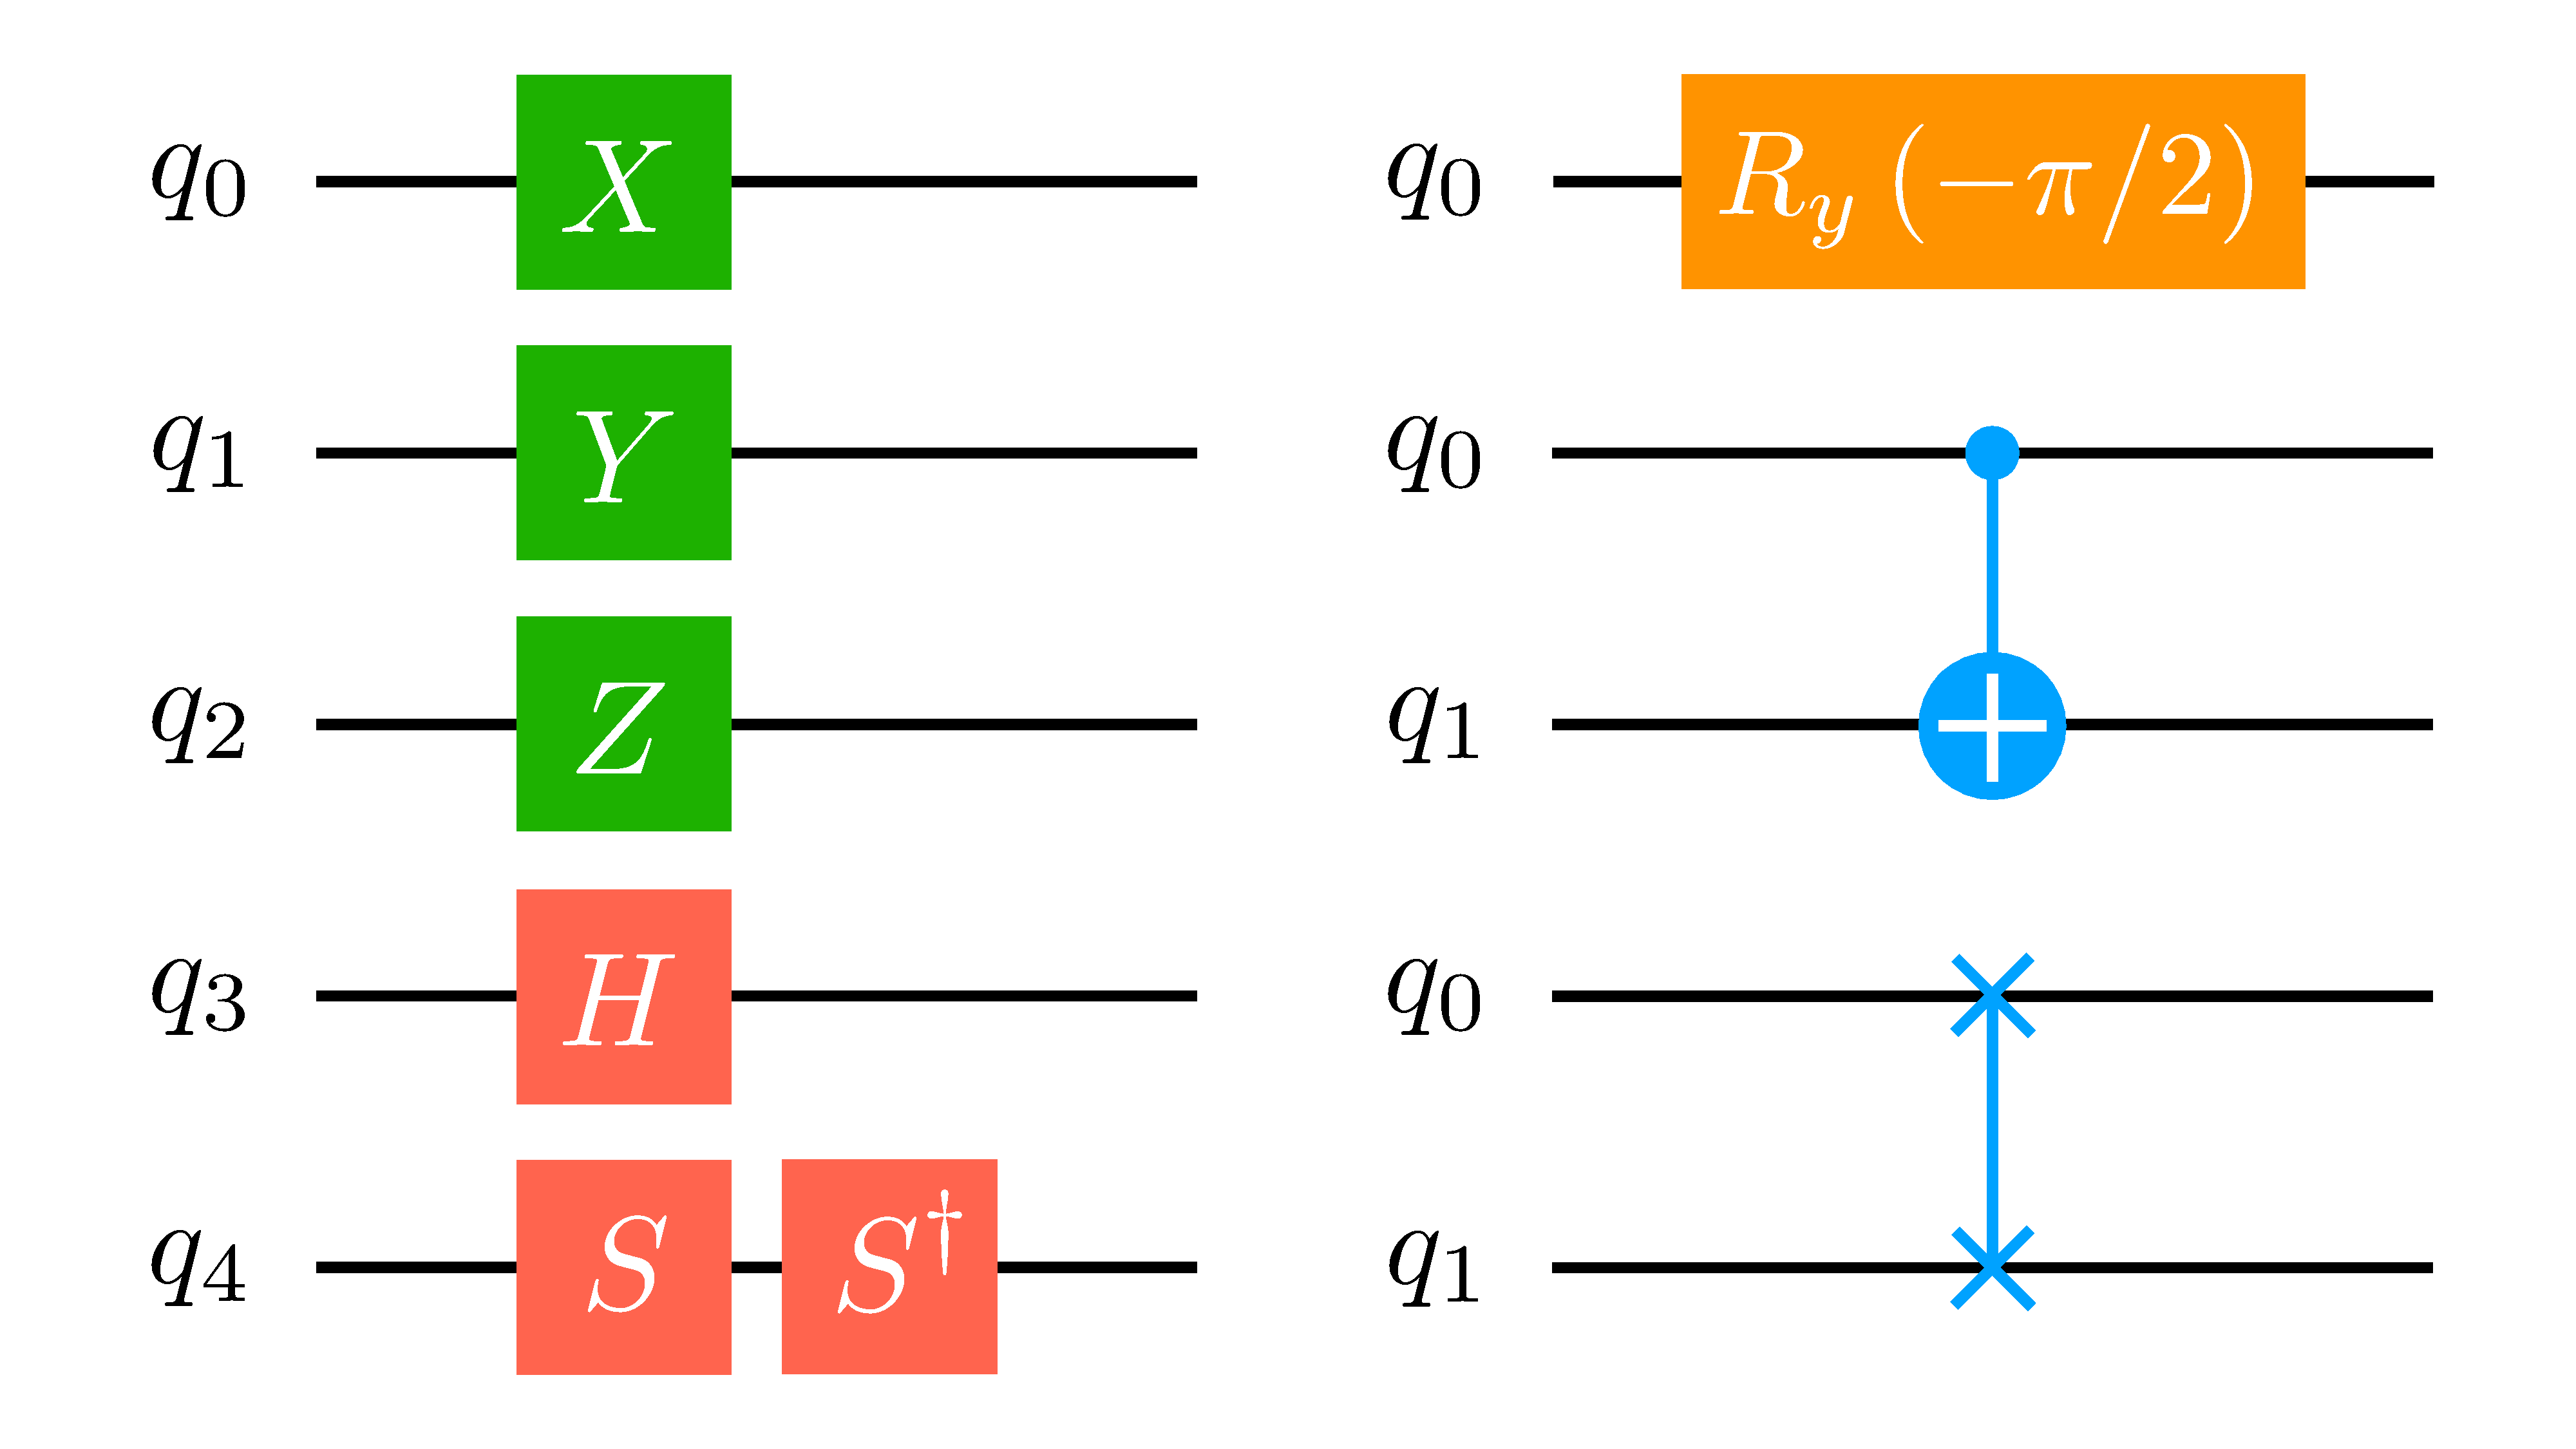
\includegraphics[width=.40\paperwidth]{Figures/quantum-background/circuit-gates-1}
		\end{center}

		\columnbreak

		\begin{center}
			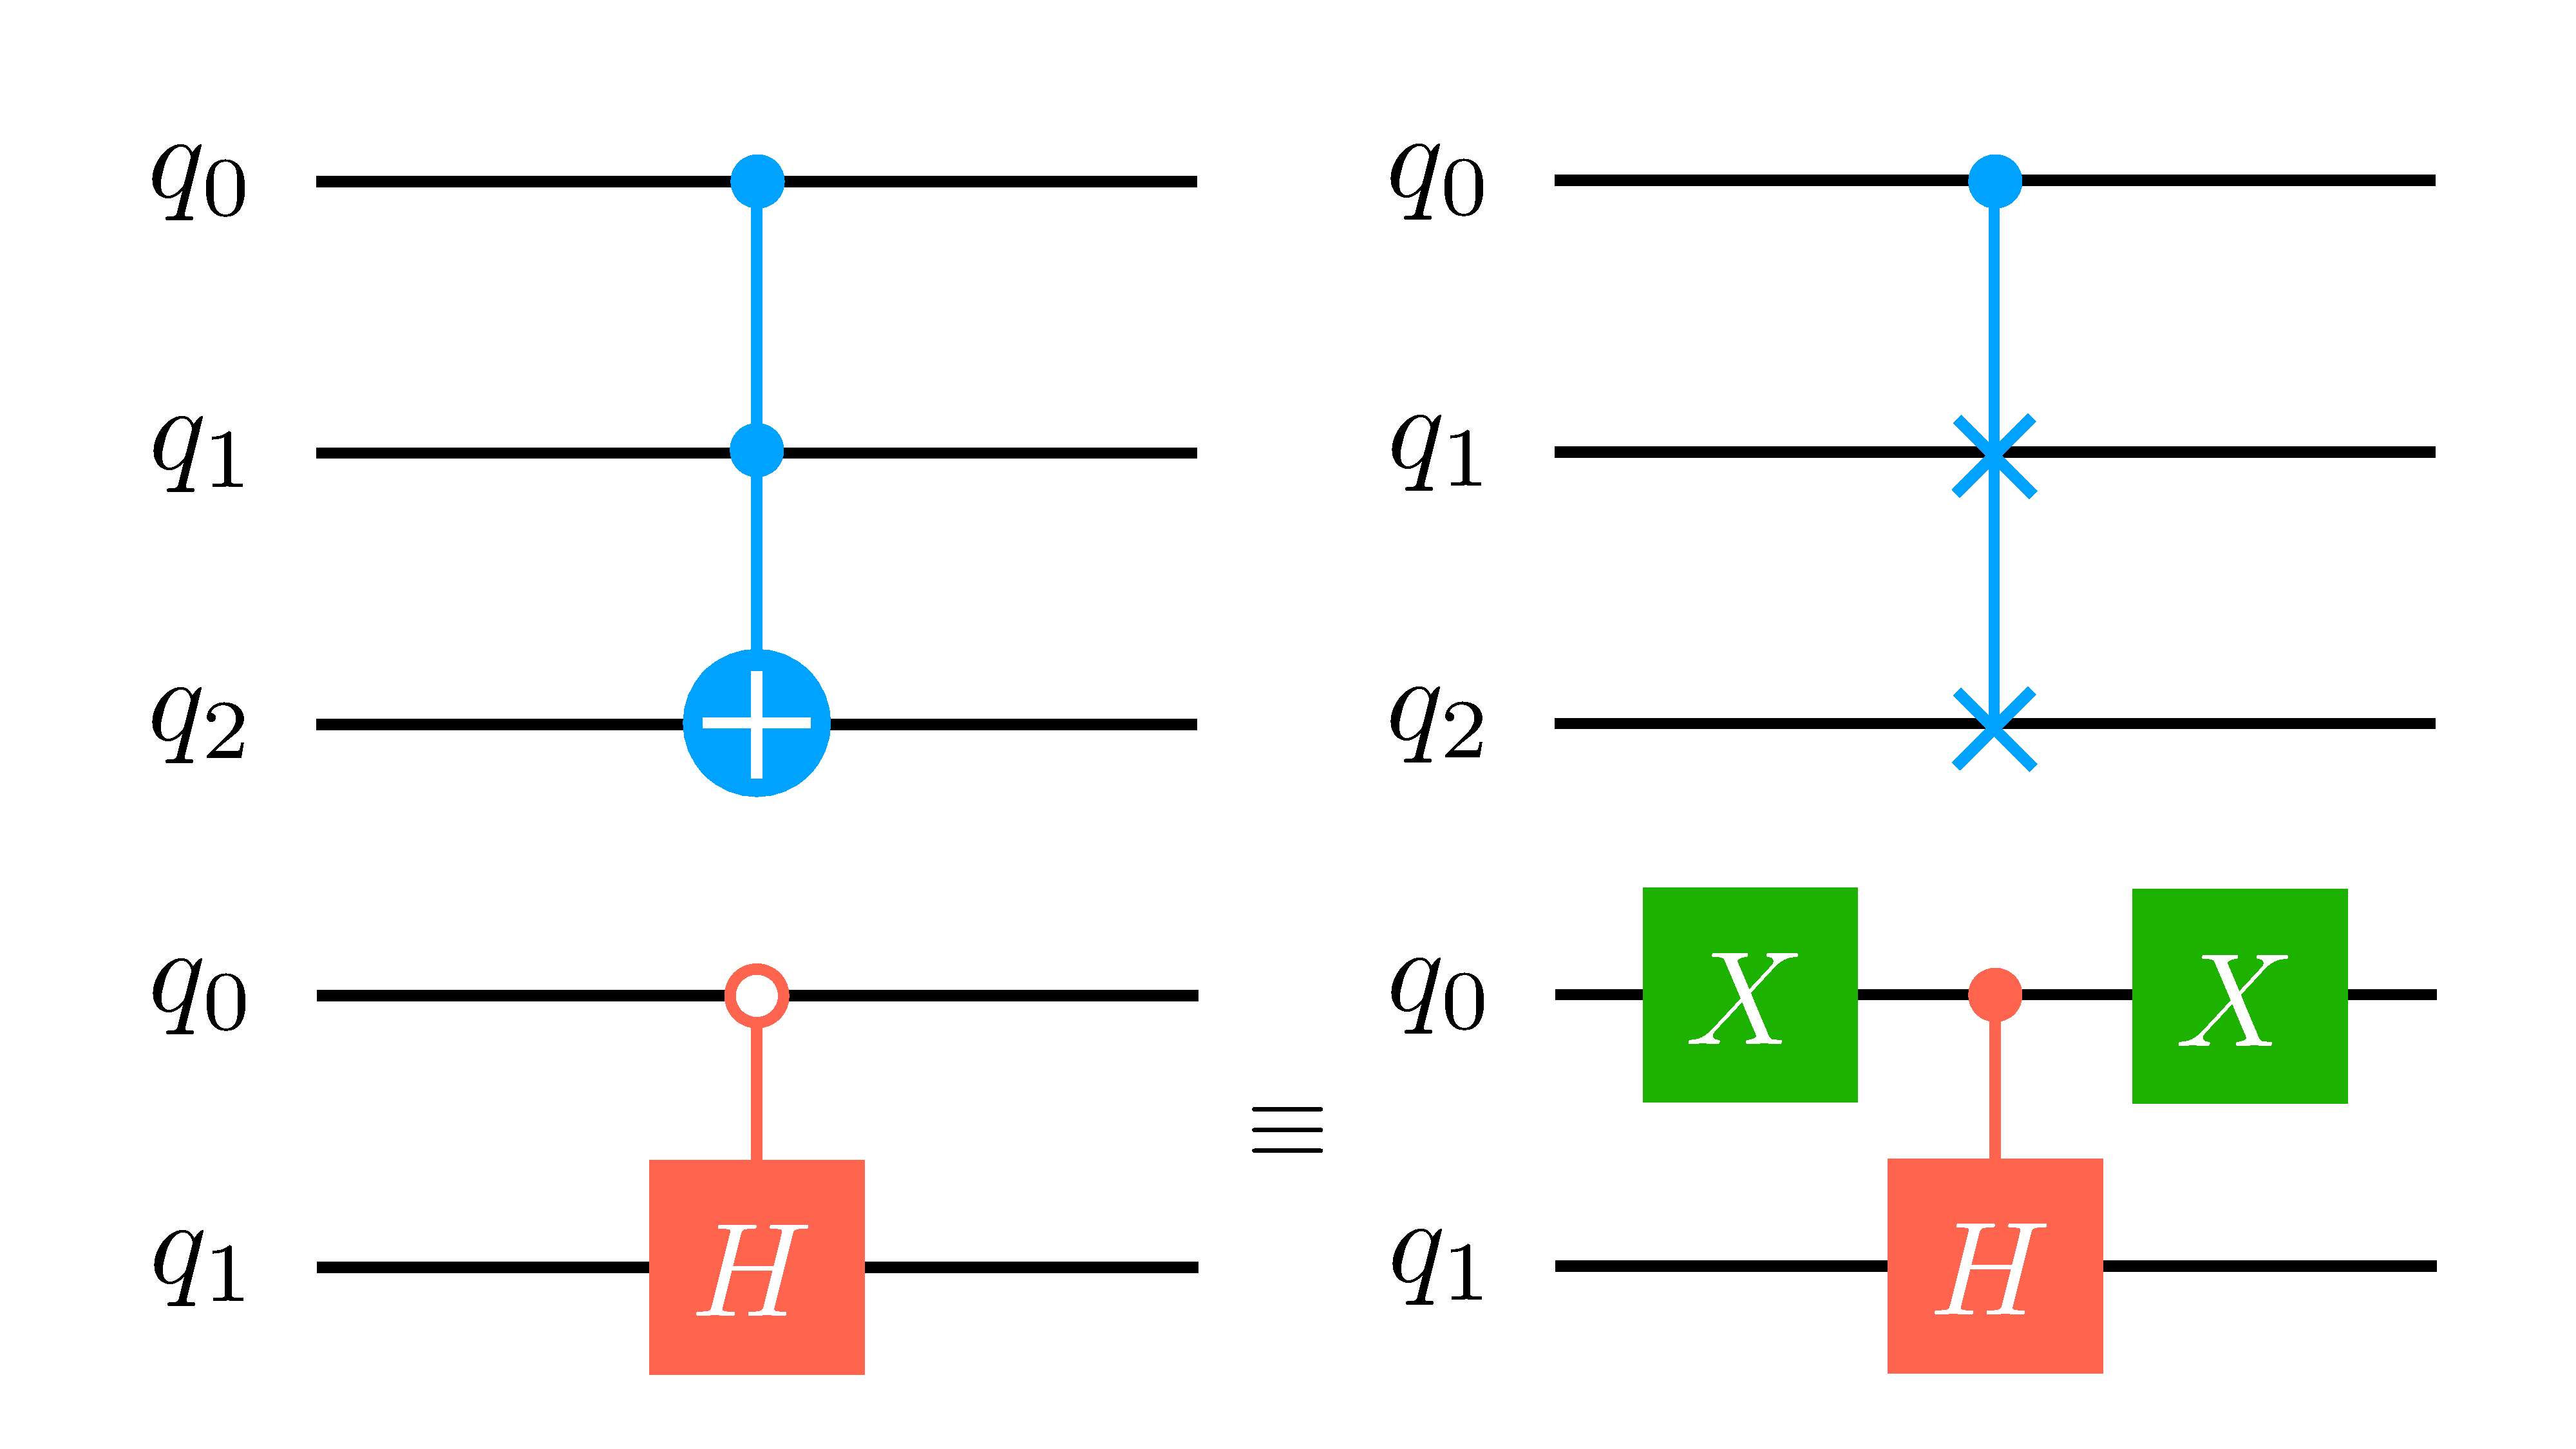
\includegraphics[width=.40\paperwidth]{Figures/quantum-background/circuit-gates-2}
		\end{center}

	\end{multicols}

\end{frame}

%% ----------------------------------------------------------------------------

\begin{frame}{Pauli measurements and the singlet state}

	The final thing that we need to know about are measurements. \textbf{Pauli measurements} are made along the three primary axes of the Bloch sphere, allowing us to calculate the expectation value of \emph{Pauli observables} (i.e. tensor product combinations of the Pauli hermitian operators):

	\begin{multicols}{2}

		\begin{center}
			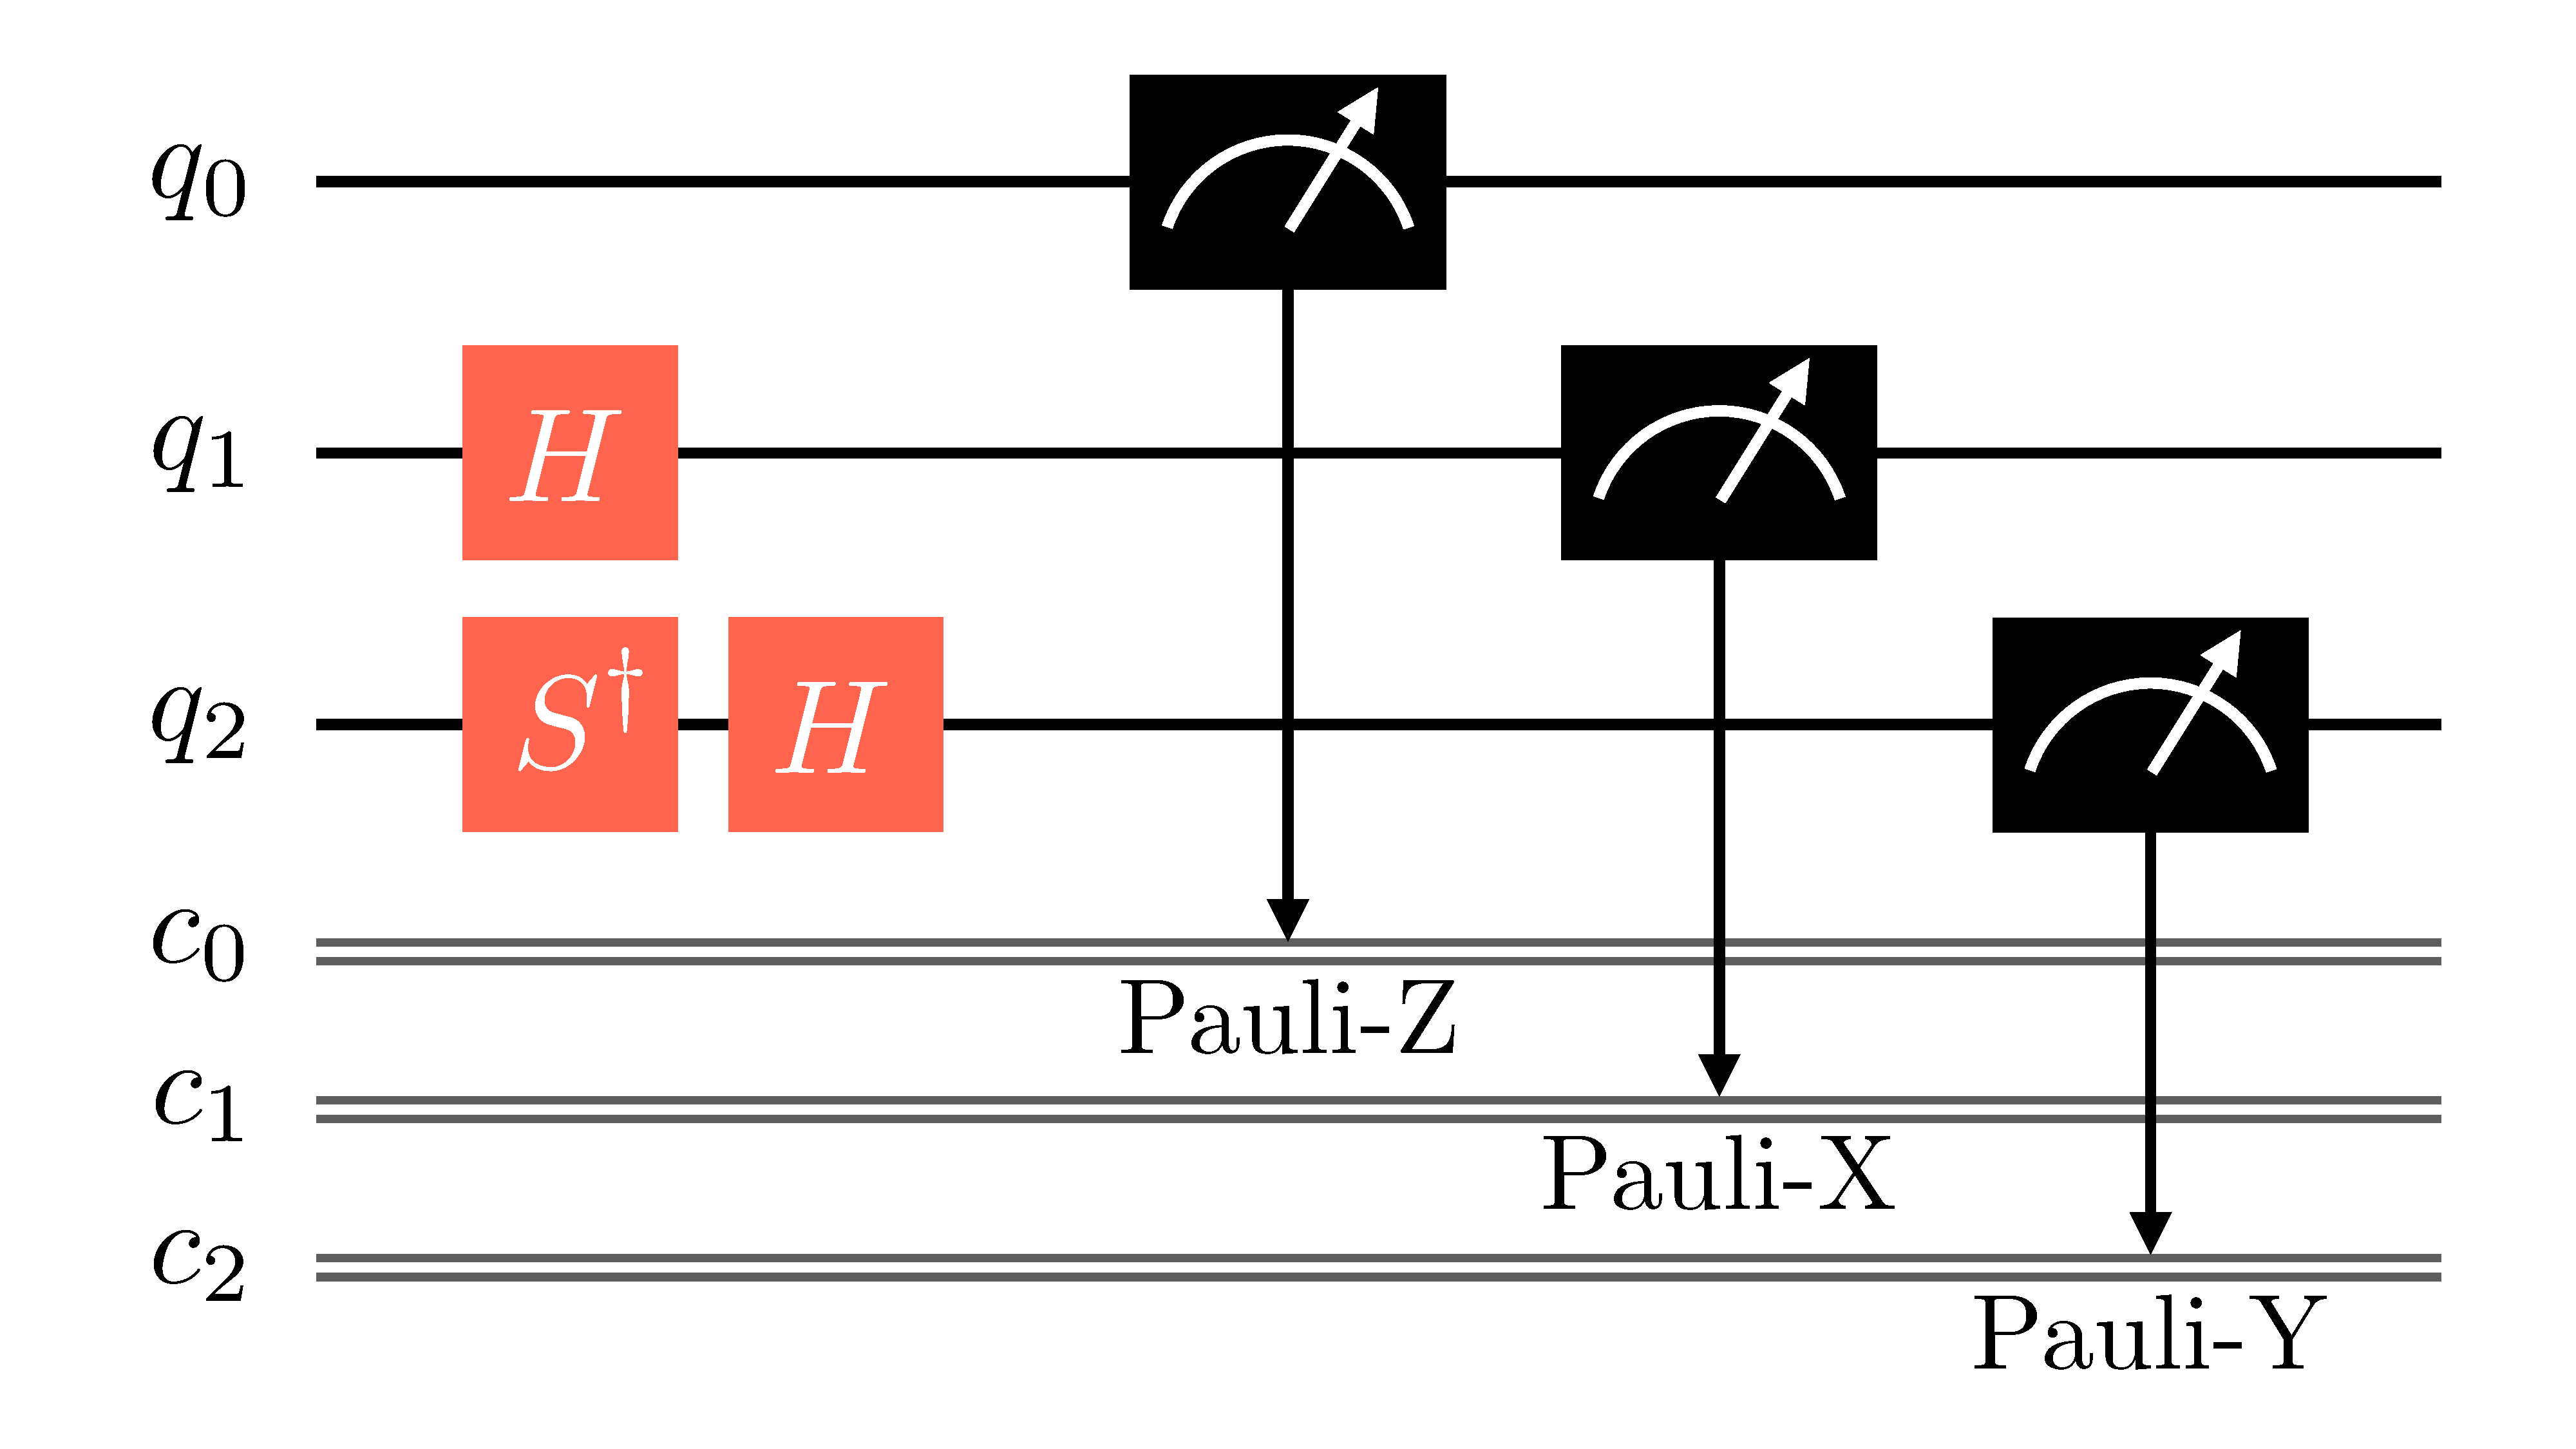
\includegraphics[width=.40\paperwidth]{Figures/quantum-background/circuit-gates-pauli}
		\end{center}

		\columnbreak

		\pause
		\begin{center}
			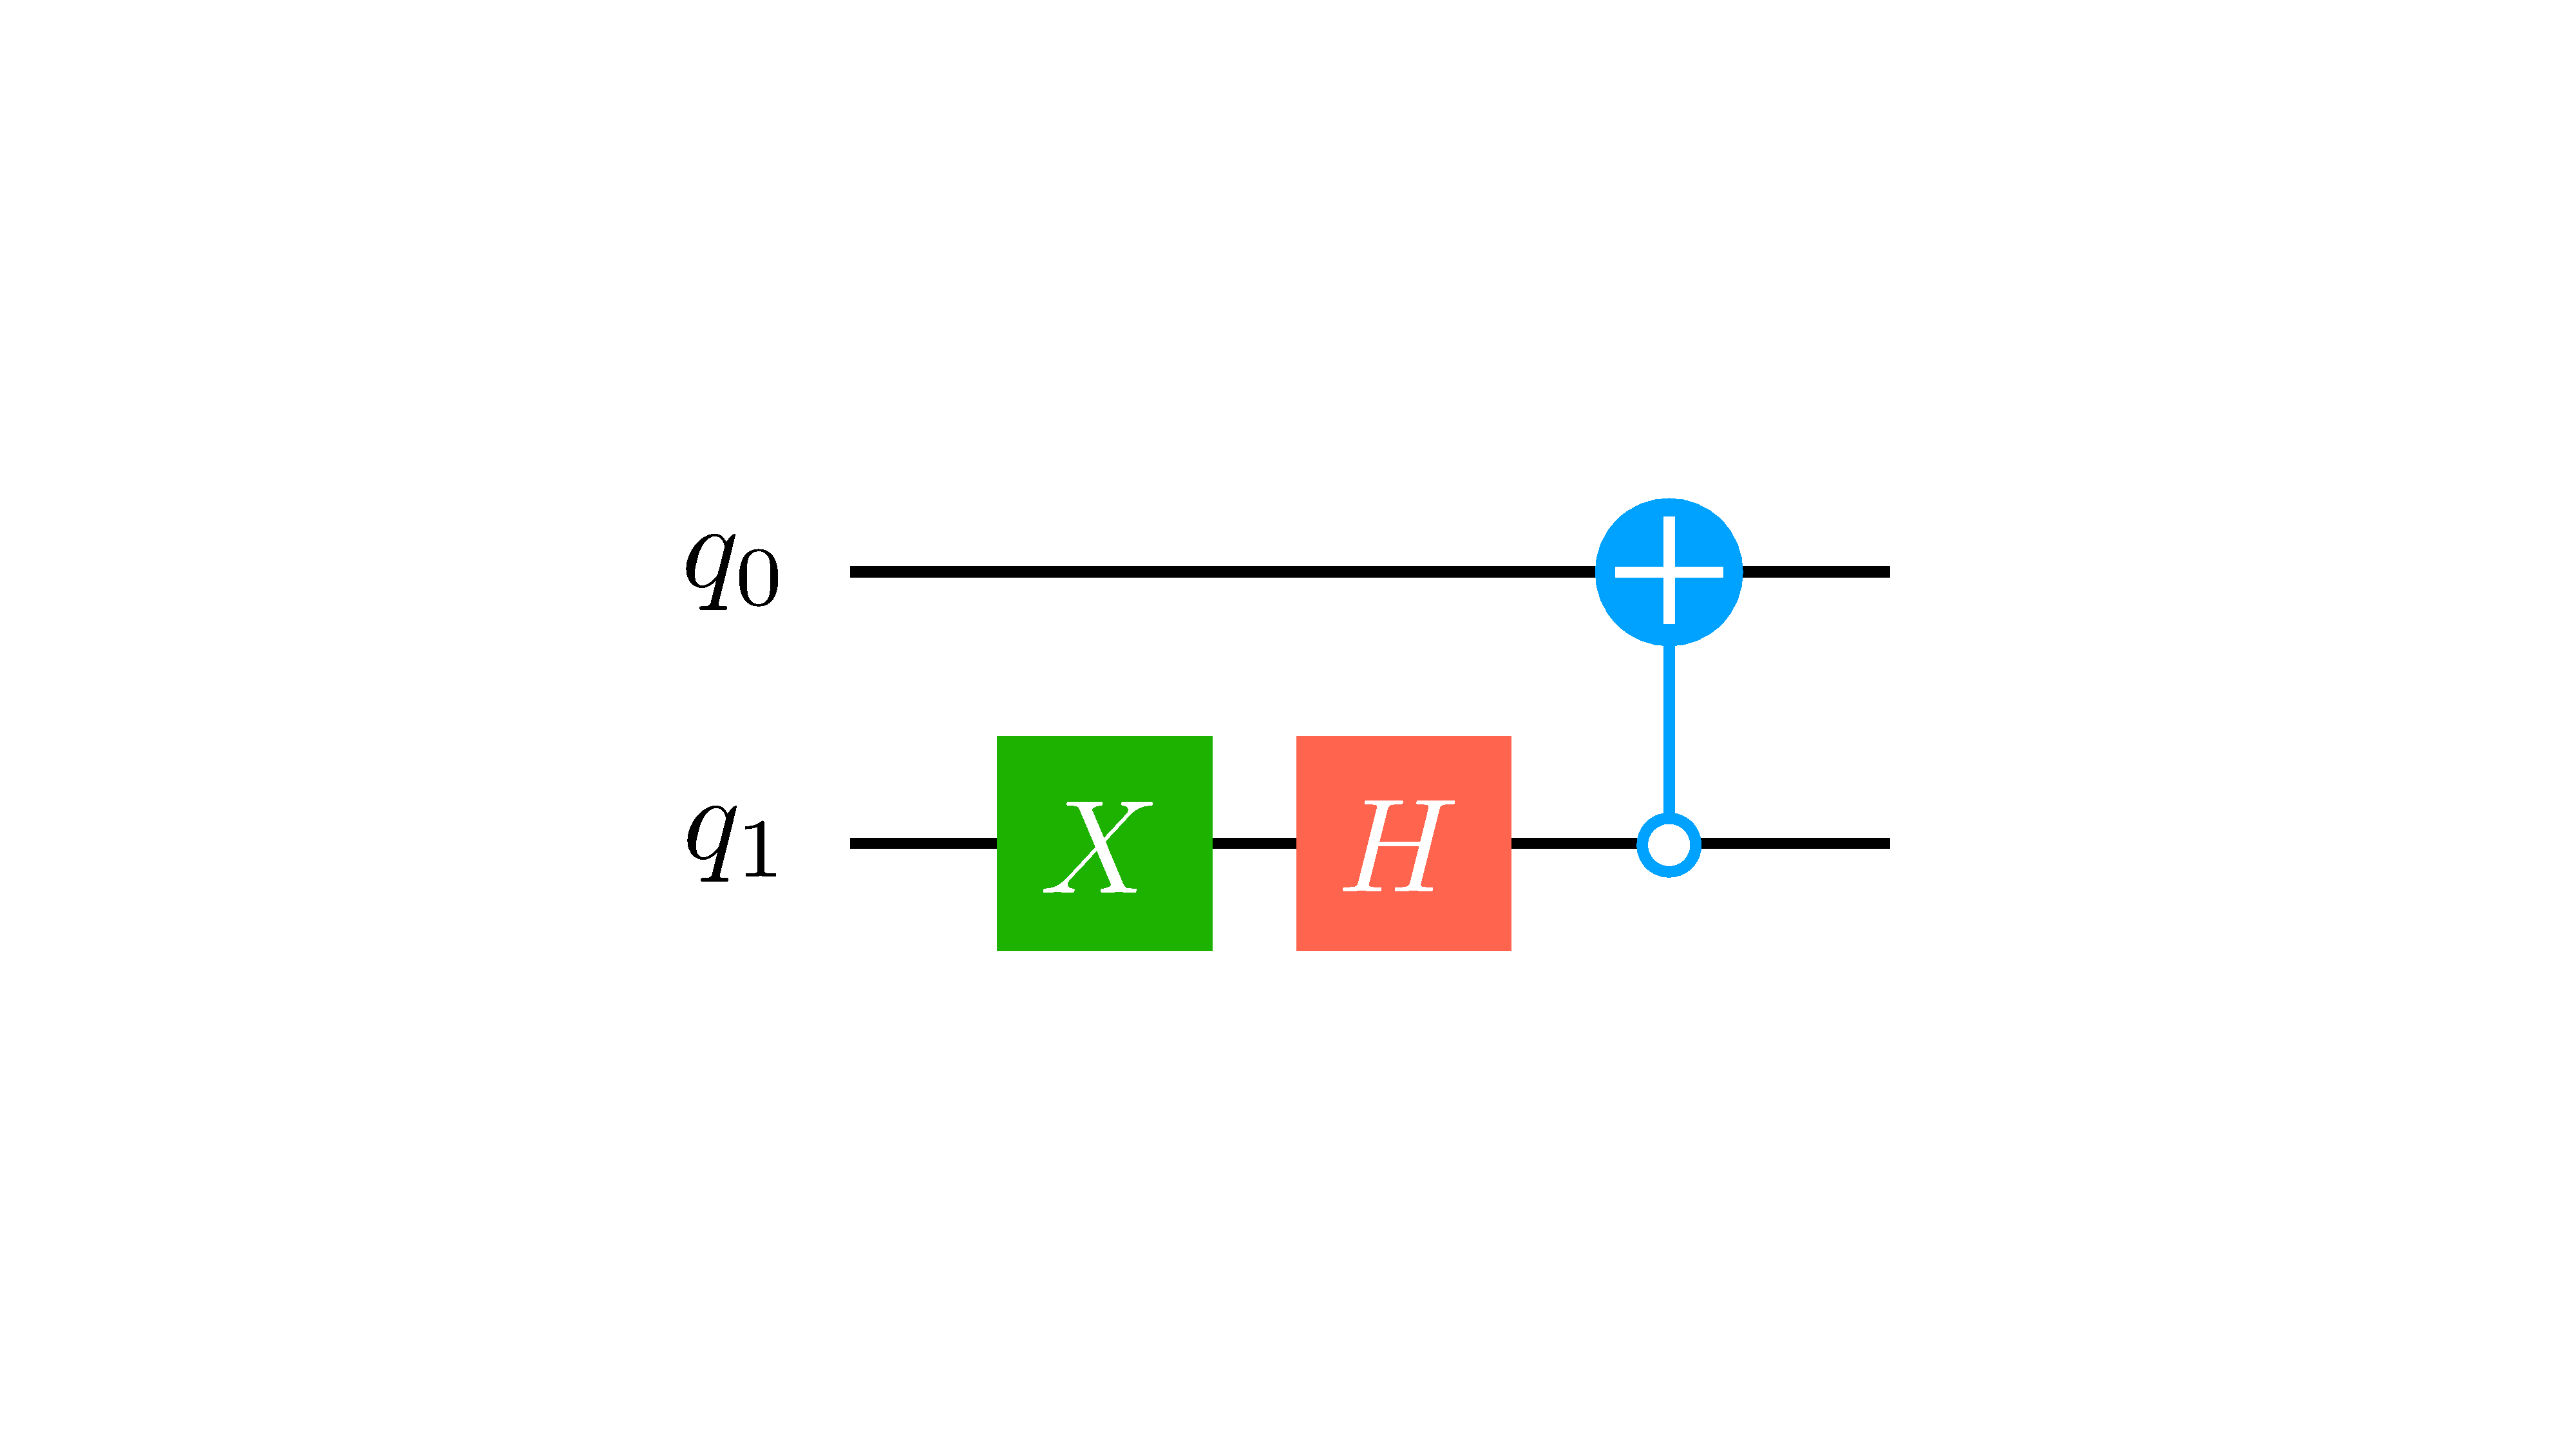
\includegraphics[width=.40\paperwidth]{Figures/quantum-background/circuit-gates-singlet}\\ \vspace{-2em}
			$\ket{\text{\small singlet}} \defeq \frac{\ket{01}-\ket{10}}{\sqrt{2}}$
		\end{center}

	\end{multicols}

\end{frame}

%% ----------------------------------------------------------------------------

\begin{frame}[allowframebreaks]{Deutsch-Jozsa algorithm}

	\begin{multicols}{2}

		\textbf{Deutsch’s problem} says that we are given a function $f: \qty{0,1}^n \ra \qty{0,1}$, and are told that the function is either constant or balanced (i.e. half of the inputs return 0 and the other half 1). The goal is to determine, with the smallest number of evaluations possible, whether the given function is one kind or the other.

		\columnbreak

		\begin{center}
			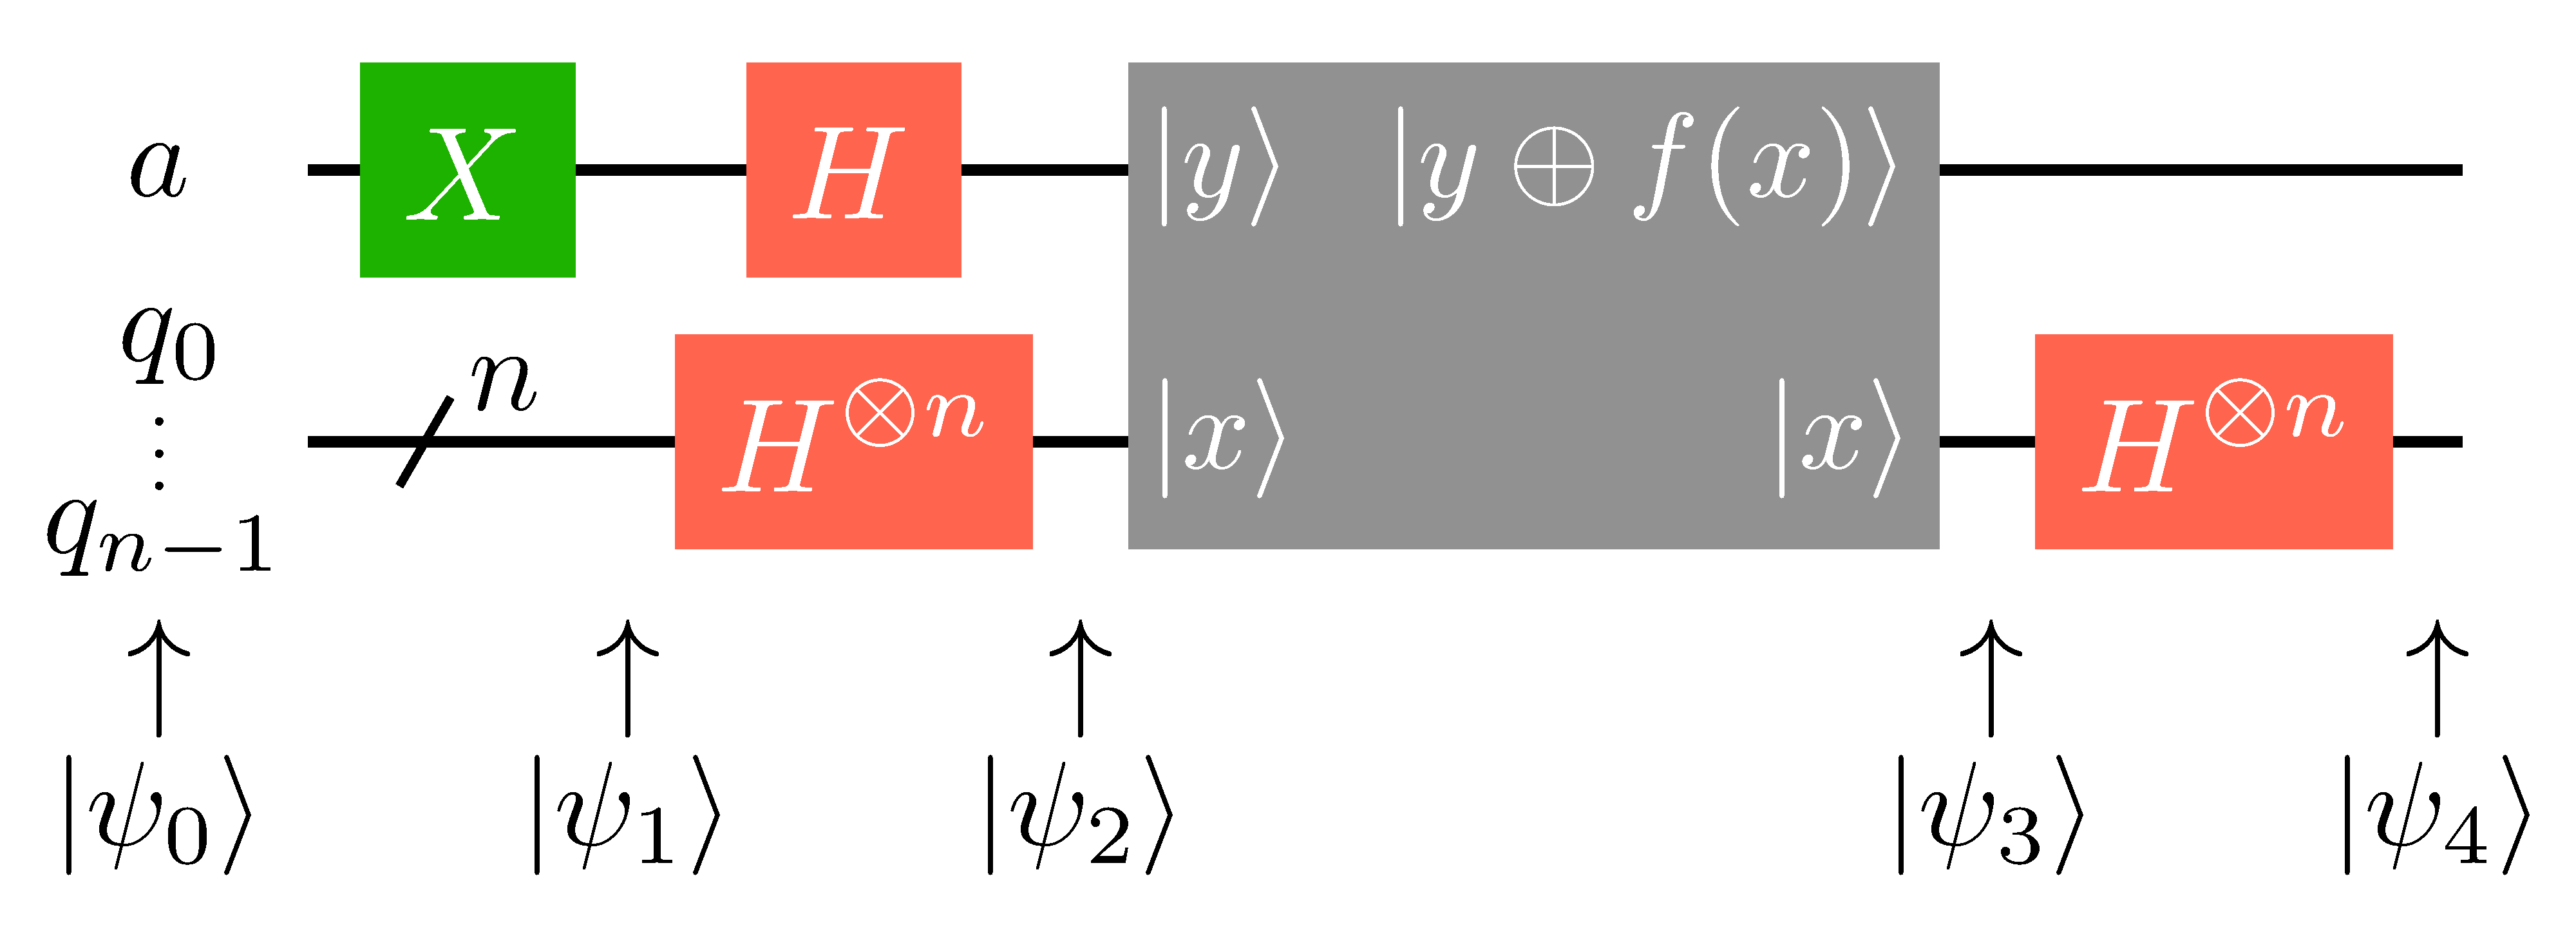
\includegraphics[width=.40\paperwidth]{Figures/quantum-background/deutsch-jozsa-algorithm}
		\end{center}

	\end{multicols}

	Using classical resources the only way to solve this problem is to repeatedly evaluate the function for different inputs. In the worst case scenario, we will need to perform $2^n/2+1$ evaluations, since it is always possible to obtain $2^n/2$ times the same number even if the function is balanced. However, making use of quantum superposition, we can find a way to solve this problem with just one evaluation. The key as to why this is possible is quantum superposition. By evaluating the target function for a superposition state, we are evaluating it simultaneously for all possible inputs. This is sometimes referred to as \textbf{quantum parallelism}.

\break

	The solution to this problem as expressed by the quantum circuit in the previous slide is known as the \textbf{Deutsch-Jozsa algorithm}:

	\begin{multicols}{2}

		\begin{gather*}
		  \ket{\psi_0} = \ket{0}^{\otimes \qty(n+1)} \\[10pt]
		  \ket{\psi_1} = \ket{0}^{\otimes n} \ket{1} \\[10pt]
			H^{\otimes n} \ket{x} =
		    \sum_{z \in \qty{0,1}^n} (-1)^{x \cdot z}
				\frac{\ket{z}}{\sqrt{2^n}} \\[10pt]
			\ket{\psi_2} =
		    \sum_{x \in \qty{0,1}^n} \frac{\ket{x}}{\sqrt{2^n}}
		    \qty[\frac{\ket{0}-\ket{1}}{\sqrt{2}}]
		\end{gather*}

		\columnbreak

		\begin{gather*}
		  \frac{\ket{0 \oplus f(x)}-\ket{1 \oplus f(x)}}{\sqrt{2}} =
		    (-1)^{f(x)} \frac{\ket{0}-\ket{1}}{\sqrt{2}} \\[10pt]
			\ket{\psi_3} =
		    \sum_{x \in \qty{0,1}^n} \frac{(-1)^{f(x)} \ket{x}}{\sqrt{2^n}}
		    \qty[\frac{\ket{0}-\ket{1}}{\sqrt{2}}] \\[10pt]
			\ket{\psi_4} =
		    \sum_{\substack{x \in \qty{0,1}^n \\ z \in \qty{0,1}^n}}
		    \frac{(-1)^{x \cdot z +f(x)} \ket{z}}{2^n}
		    \qty[\frac{\ket{0}-\ket{1}}{\sqrt{2}}]
		\end{gather*}

	\end{multicols}

\end{frame}

%% ----------------------------------------------------------------------------

\begin{frame}[allowframebreaks]{Quantum Fourier transform}

	The usual \textbf{Discrete Fourier Transform} (DFT) can be expressed as:

	\medskip

	\begin{align*}
	  \ket{j} \qra&
				\frac{1}{\sqrt{N}} \sum_{k=0}^{N-1} \exp[2\pi i \frac{jk}{N}] \ket{k} \\
	    =& \frac{1}{2^{n/2}} \sum_{k_{n-1}=0}^{1} \cdots \sum_{k_{0}=0}^{1}
	      \exp[2\pi ij \qty(\sum_{l=0}^{n-1} k_{l} 2^{l-n})]
	      \ket{\bin k_{n-1} \dots k_{0}} \\
	    =& \frac{1}{2^{n/2}} \sum_{k_{n-1}=0}^{1} \cdots \sum_{k_{0}=0}^{1}
	      \qty{ \bigotimes_{l=1}^{n} \exp[2\pi ij k_{n-l} 2^{-l}]
	      \ket{k_{n-l}} } \\
	    =& \frac{1}{2^{n/2}} \bigotimes_{l=1}^{n}
	      \qty{ \sum_{k_{n-l}=0}^{1} \exp[2\pi ij k_{n-l} 2^{-l}] \ket{k_{n-l}} }
	    = \frac{1}{2^{n/2}} \bigotimes_{l=1}^{n}
	      \qty{ \ket{0} + \exp[2\pi ij 2^{-l}] \ket{1} }
	\end{align*}

\break

	\begin{gather*}
		\ket{j} \ra
			\frac{
				\qty{\ket{0}+ e^{2\pi i \qty(\bin.j_{0})} \ket{1}} \otimes
				\qty{\ket{0}+ e^{2\pi i \qty(\bin.j_{1}j_{0})} \ket{1}} \otimes
				\cdots \otimes
				\qty{\ket{0} + e^{2\pi i \qty(\bin.j_{n-1}j_{n-2} \dots j_{0})} \ket{1}}
			}{2^{n/2}} \\[10pt]
		R_{k} \defeq \mqty[1 & 0 \\ 0 & e^{2\pi i/2^k}]
	\end{gather*}

	\vspace{-2em}

	\begin{center}
		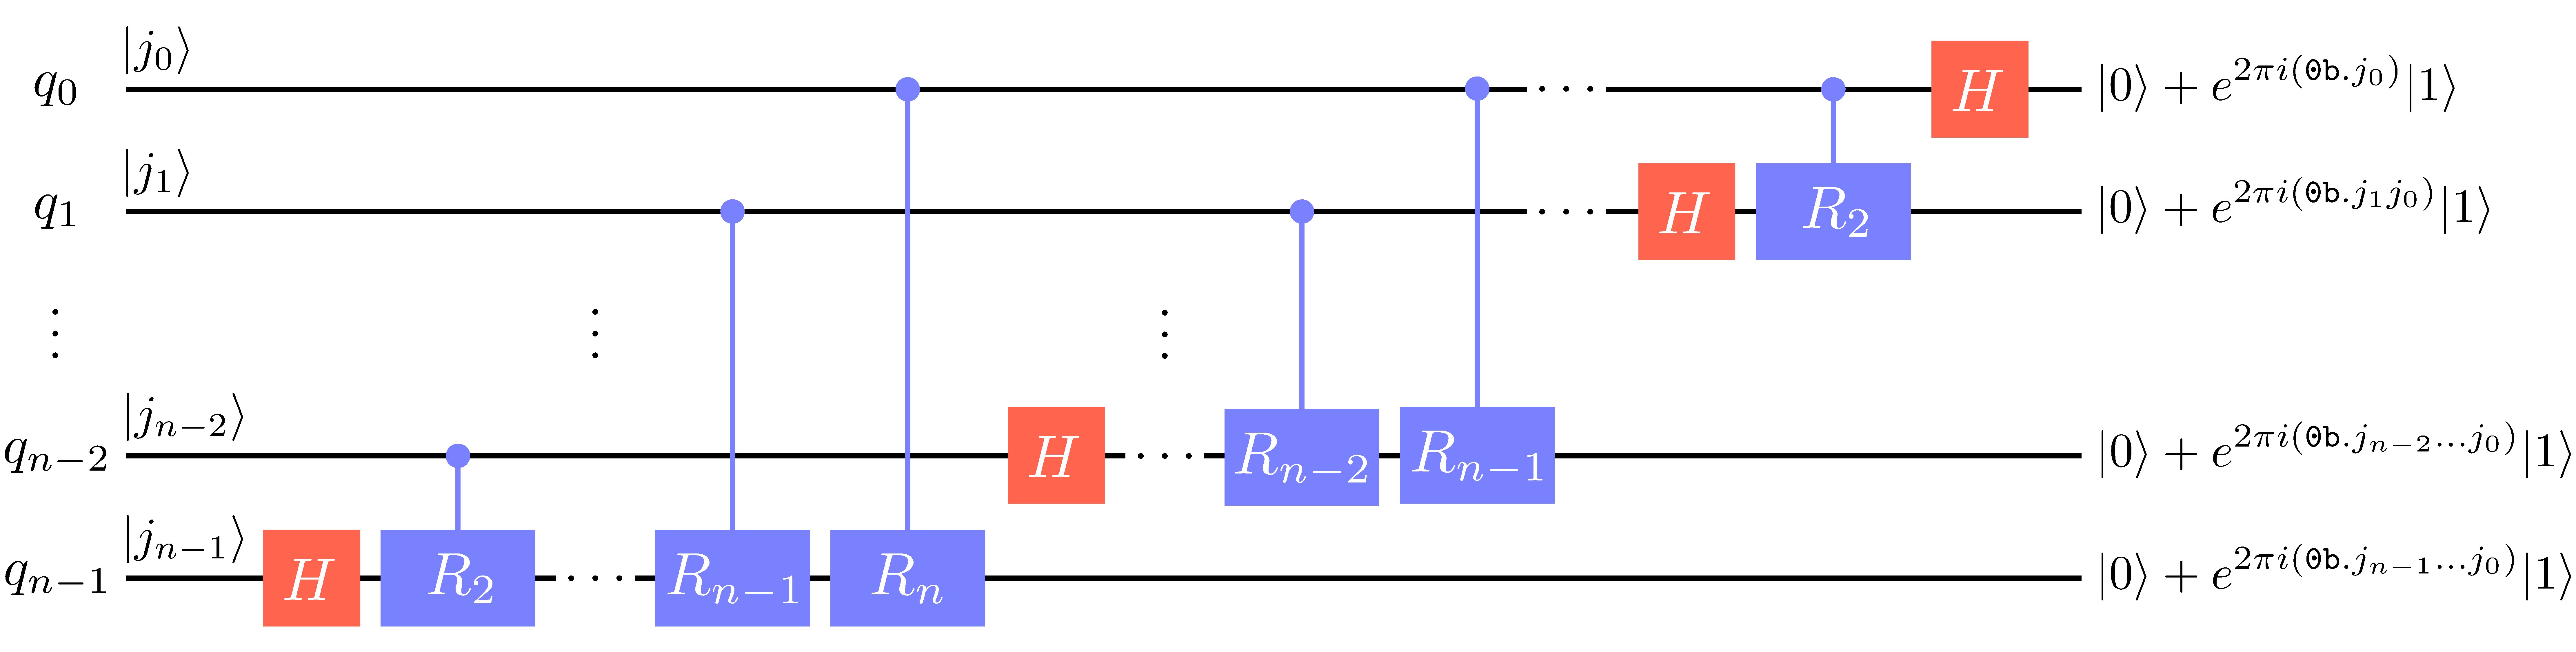
\includegraphics[width=.80\paperwidth]{Figures/quantum-background/quantum-fourier-transform}
	\end{center}

\break

	We can now compare the complexity of this algorithm with its best classical counterparts. This is done by counting the number of gates in the circuit, where we have to remember the final SWAP gates omitted in the representation.

	\begin{multicols}{2}
	\begin{centering}

		\underline{\textbf{FAST FOURIER TRANSFORM}}\\
		\medskip
		$N\log_2 N \equiv \Theta\qty(n2^n)$

		\columnbreak

		\underline{\textbf{QUANTUM FOURIER TRANSFORM}}\\
		\medskip
		$\sum_{k=1}^{n}k + \frac{n}{2} =
			\frac{n\qty(n+1)}{2} + \frac{n}{2} \equiv \Theta\qty(n^2)$

	\end{centering}
	\end{multicols}

	Nonetheless, this technique cannot be used directly for computing the target transform; since we do not know how to recover the individual amplitudes from the quantum states. On top of that, there is no efficient general method for preapring the states to be transformed. This is a great example of an algorithm that presents huge savings compared to its classical analogs, but which cannot be generally used as much as we would like to due to our inability to extract the desirerd information. In some instances however, we can profit from this method to great deeds ---mainly as part of bigger algorithms. An important application is \textbf{Shor's factoring algorithm}, which can be used for efficiently finding the prime decomposition of any given number.

\end{frame}

%% ----------------------------------------------------------------------------

\subsection{Applications}

\begin{frame}{Applications}

	Generally speaking, quantum computing is thought to be able to outperform classical processors, but not for all tasks. This raises the important question of determining which problems are easy to solve using quantum logic while remaining hard for classical approaches. As a matter of fact, we do not fully understand the extent to which there are problems of this kind; and many of the ones we suspect to be good candidates have no formal proof to back them up.\pause~So far, some of the applications that have been found are:

	\begin{multicols}{3}

		\begin{itemize}
			\item Cryptography
			\item Secure communications
			\item Quantum randomness
		\end{itemize}

		\columnbreak

		\begin{itemize}
			\item Quantum sensing
			\item Optimization
			\item Algebra
		\end{itemize}

		\columnbreak

		\begin{itemize}
			\item Machine learning
			\item Quantum games
			\item Quantum simulation
		\end{itemize}

	\end{multicols}

	\pause

	Quantum physics ---especially Quantum Field Theory--- is the ideal place to look for (relevant) problems which can be solved on a quantum computer while remaining intractable for classical machines; that also makes it the best choice for analyzing the computational power behind this new paradigm.

\end{frame}


%% ----------------------------------------------------------------------------
%% ----------------------------------------------------------------------------

\section{Solving the NJL model in $1+1$ dimensions}

%% ----------------------------------------------------------------------------

% \subsection{Analytical solution}

%% ----------------------------------------------------------------------------

\subsection{Lattice formulation}

%% ----------------------------------------------------------------------------

\subsection{Fermion-qubit mapping}

%% ----------------------------------------------------------------------------

\subsection{Space parametrization and state preparation}

%% ----------------------------------------------------------------------------

\subsection{Ground state energy}


%% ----------------------------------------------------------------------------
%% ----------------------------------------------------------------------------

\section{Conclusions and prospective work}


%% ----------------------------------------------------------------------------
%% BACK-MATTER
%% ----------------------------------------------------------------------------

\section{Bibliography}
%	\begin{frame}[allowframebreaks]{Bibliography}
\begin{frame}{Bibliography}

	\begin{thebibliography}{9}
		\setbeamertemplate{bibliography item}[online]
	\bibitem{hayden} \textbf{Hayden, P.} \emph{Quantum Computational Universe}
		\setbeamertemplate{bibliography item}[book]
	\bibitem{susskind_book} \textbf{Susskind, L. \& Friedman A.} \emph{Quantum Mechanics: The Theoretical Minimum}
		\setbeamertemplate{bibliography item}[book]
	\bibitem{nielsen} \textbf{Nielsen M.A. \& Chuang I.L.} \emph{Quantum Computation and Quantum Information}
		\setbeamertemplate{bibliography item}[article]
	\bibitem{ladd} \textbf{Lykken J.} \emph{Quantum Technologies for Quantum Science}
		\setbeamertemplate{bibliography item}[book]
	\bibitem{mermin} \textbf{Mermin N.D.} \emph{Quantum Computer Science: An Introduction}
		\setbeamertemplate{bibliography item}[article]
	\bibitem{ladd} \textbf{Ladd T.D. (et al.)} \emph{Quantum Computing}

	\end{thebibliography}

	\vspace{20pt}
	\begin{small}
	\begin{center}{
	\color{gray}
		\emph{"The only thing demonstrated by an impossibility proof is a lack of imagination."} \\
		\textbf{– John Stewart Bell –} }
	\end{center}
	\end{small}
\end{frame}

\FinalFrame

\end{document}
